% BEGIN LICENSE BLOCK
% Version: CMPL 1.1
%
% The contents of this file are subject to the Cisco-style Mozilla Public
% License Version 1.1 (the "License"); you may not use this file except
% in compliance with the License.  You may obtain a copy of the License
% at www.eclipse-clp.org/license.
% 
% Software distributed under the License is distributed on an "AS IS"
% basis, WITHOUT WARRANTY OF ANY KIND, either express or implied.  See
% the License for the specific language governing rights and limitations
% under the License. 
% 
% The Original Code is  The ECLiPSe Constraint Logic Programming System. 
% The Initial Developer of the Original Code is  Cisco Systems, Inc. 
% Portions created by the Initial Developer are
% Copyright (C) 2006 Cisco Systems, Inc.  All Rights Reserved.
% 
% Contributor(s): Helmut Simonis, Parc Technologies
% 
% END LICENSE BLOCK

\documentclass[a4paper,12pt]{report}
\usepackage{hevea}
\usepackage{alltt}
\usepackage{graphics}
\usepackage{makeidx}
%\usepackage{html}
\usepackage{tocbibind}
\usepackage{hyperref}
\usepackage{../texinputs/eclipse}
%
% $Id: sepiachiphtml.tex,v 1.10 2016/07/28 03:34:36 jschimpf Exp $
%
% BEGIN LICENSE BLOCK
% Version: CMPL 1.1
%
% The contents of this file are subject to the Cisco-style Mozilla Public
% License Version 1.1 (the "License"); you may not use this file except
% in compliance with the License.  You may obtain a copy of the License
% at www.eclipse-clp.org/license.
%
% Software distributed under the License is distributed on an "AS IS"
% basis, WITHOUT WARRANTY OF ANY KIND, either express or implied.  See
% the License for the specific language governing rights and limitations
% under the License.
%
% The Original Code is  The ECLiPSe Constraint Logic Programming System.
% The Initial Developer of the Original Code is  Cisco Systems, Inc.
% Portions created by the Initial Developer are
% Copyright (C) 2006 Cisco Systems, Inc.  All Rights Reserved.
%
% Contributor(s):
%
% END LICENSE BLOCK

% This is not the original sepiachip.sty,
% but a drastically simplified one.
%

\newcommand{\eclipseversion}{7.2}

% characters for indexing ? needed for a HeVeA bug
\newcommand*{\query}{?}
\newcommand*{\atsym}{@}
\newcommand*{\cutsym}{!}

% Like index, but in tt font
\newcommand*{\indextt}[1]{\index{#1@\texttt{#1}}}

\newcommand*{\newitem}[1]{\item[#1]}

\newcommand*{\bipnoidx}[1]{\textbf{#1}}
\newcommand*{\bip}[1]{\bipnoidx{#1}\indextt{#1}}

%\newcommand{\biprefnoidx}[2]{\latex{{\bf #1}}\html{\htmladdnormallink{#1}{#2}}}
\newcommand*{\biprefnoidx}[2]{\ahref{#2}{\textbf{#1}}}
\newcommand*{\biprefni}[2]{\biprefnoidx{#1}{#2}}
\newcommand*{\bipref}[2]{\biprefnoidx{#1}{#2}\indextt{#1}}

\newcommand*{\biptxt}[2]{\bipnoidx{#1}\indextt{#2}}
\newcommand*{\txtbip}[2]{\bipnoidx{#1}\indextt{#1}}

\newcommand*{\biptxtrefni}[3]{\biprefnoidx{#1}{#3}}
\newcommand*{\biptxtref}[3]{\biprefnoidx{#1}{#3}\indextt{#2}}

\newcommand*{\txtbiprefni}[3]{\biprefnoidx{#1}{#3}}
\newcommand*{\txtbipref}[3]{\txtbiprefni{#1}{}{#3}\indextt{#1}}

% Put this word in the text, but also index it:
\newcommand*{\Index}[1]{#1\index{#1}}
% Ditto, but index in textt:
\newcommand*{\Indextt}[1]{#1\indextt{#1}}

% A word/phrase that we are talking about, not just a part of the sentence:
\newcommand*{\about}[1]{\emph{#1}}
% Ditto, with an index entry:
\newcommand*{\aboutidx}[1]{\about{#1}\index{#1}}

% Chapter name
\newcommand*{\chapname}[1]{\emph{#1}}

% Example name
\newcommand*{\examplename}[1]{\emph{#1}}

% Tool name
\newcommand*{\toolname}[1]{\emph{#1}}

% The first, defining occurrence of the name of a concept etc.:
\newcommand*{\defnotion}[1]{\textbf{#1}\index{#1}}
% Ditto with a different index entry:
\newcommand*{\defnotioni}[2]{\textbf{#1}\index{#2}}
% Ditto without an index entry:
\newcommand*{\defnotionni}[1]{\textbf{#1}}

% Concrete notation, also a very short fragment of a program embedded in the
% text, a concrete file name etc.
\newcommand*{\notation}[1]{\texttt{#1}}
% Ditto, with an index entry:
\newcommand*{\notationidx}[1]{\notation{#1}\indextt{#1}}

% A pattern, i.e., notation that is not concrete:
\newcommand*{\pattern}[1]{\textsl{#1}}
% Ditto, with an index entry:
\newcommand*{\patternidx}[1]{\pattern{#1}\index{#1@\textsl{#1}}}

% Predicate specification, i.e., name/arity
\newcommand*{\predspec}[1]{\textbf{#1}}
% Ditto with an index entry:
\newcommand*{\predspecidx}[1]{\predspec{#1}\indextt{#1}}

% Predicate ``definition'', e.g., showing it with arguments patterns.
% NOTE: have to add indextt explicitly.
\newcommand*{\preddef}[1]{\textbf{#1}}

% Index entry for a library:
\newcommand*{\libidx}[1]%
{\index{#1@\textbf{#1} (library)}\index{library!\textbf{#1}}}
% Library specification, with index:
\newcommand*{\libspec}[1]{\textbf{#1}\libidx{#1}}


% Index entry for a command line option:
\newcommand*{\cmdlineoptionidx}[1]%
{\index{command line options!\notation{-#1}}%
\index{#1 (command line option)@\notation{-#1} (command line option)}}

% Index entry for a handler:
\newcommand*{\handleridx}[1]%
{\index{#1 handler@\notation{#1} handler}\index{handler!\notation{#1}}}

% Bold table column heading etc.
\newcommand*{\heading}[1]{\textbf{#1}}



\newcommand*{\vbar}{$\mid$}
\newcommand*{\uparr}{$\wedge$}
\newcommand*{\bsl}{$\backslash$}
\newcommand*{\andsy}{$/\backslash$}
\newcommand*{\orsy}{$\backslash/$}
\newcommand*{\tld}{$\sim$}
\newcommand*{\lbr}{$[$}
\newcommand*{\rbr}{$]$}
\newcommand*{\nil}{$[~]$}
\newcommand*{\lt}{$<$}
\newcommand*{\gt}{$>$}
\newcommand*{\chr}{{\sf CHR}}
\newcommand*{\chrs}{{\sf CHR}s}
\newcommand*{\eclipse}{ECL$^i$PS$^e$}
\newcommand*{\tkeclipse}{TkECL$^i$PS$^e$}
\newcommand*{\sepia}{SEPIA}



%-------------------------------
%
% @(#)umsdebuggercomms.tex	1.3 93/03/29
%
\newenvironment{descr}[1]
{\begin{list}{}{\setlength{\leftmargin}{#1}}}{\end{list}}

% Index entry for a debugger command:
\newcommand*{\dbgcmdidx}[2]{\dbgcmdidxPlus{#1}{#1}{#2}}
% Ditto when the indexing entry is different from the one shown,
% e.g., \dbgcmdidxPlus{$<$}{<}{print depth}:
\newcommand*{\dbgcmdidxPlus}[3]%
{\index{#1---#3 (debugger cmd)@\notation{#2}---#3 (debugger cmd)}%
\index{debugger command!\notation{#2}}}

\newcommand*{\cmd}[2]%
{\item[\textbf{#1}\hfill]\textbf{#2}\dbgcmdidx{#1}{#2}}

\newcommand*{\ncmd}[2]{\item[\textit{n} \textbf{#1}\hfill]\textbf{#2}%
\dbgcmdidx{#1}{#2}}

\newcommand*{\mcmd}[2]{\mcmdPlus{#1}{#1}{#2}}

\newcommand*{\mcmdPlus}[3]{\item[\textbf{#1} \textit{par}\hfill]\textbf{#3}%
\dbgcmdidxPlus{#1}{#2}{#3}}

\newcommand*{\nmcmd}[2]{\item[{\it n\bf #1 {\it par}} \hfill] {\bf #2}%
\dbgcmdidx{#1}{#2}}
%-------------------------------


\let\ifonline=\iffalse


%
% \techReport
%
\usepackage{pstricks}
\newcommand{\techReport}[3]{
\thispagestyle{empty}
\begin{center}\fbox{\large TECHNICAL REPORT IC-PARC-#1}\end{center}
\vspace{120pt}
\begin{center}
\huge #2
\vspace{24pt} \\
\large #3
\end{center}
\vspace{\fill}
\newpage
\title{#2}
}


\makeindex
\begin{document}
\techReport{03-2}{Developing Applications with ECLiPSe}{H. Simonis\\
email: Helmut.Simonis@crosscoreop.com\\
}

%\title{Developing Applications with ECLiPSe}%
%\author{H. Simonis\\
%Parc Technologies Limited\\
%8th Floor, The Tower Building\\
%11 York Road\\
%London SE1 7NX\\
%email: Helmut.Simonis@parc-technologies.com\\
%}%
%\maketitle
\begin{abstract}
In this tutorial we provide a methodology for developing large scale 
applications with the ECLiPSe system. This methodology follows a top-down 
approach from the original problem specification to detailed implementation 
aspects of the resulting code. We concentrate on general design and 
programming aspects, and largely ignore specific problem solving 
techniques, which can be found in other tutorials. This current report 
is intended for programmers developing applications with ECLiPSe 
as well as those tasked with the maintenance of such programs.

This tutorial is based on an earlier version restricted to internal Parc Technologies use, and contains numerous corrections and improvements suggested by the ECLiPSe team. 
\end{abstract}
\pagestyle{headings}
\tableofcontents
\newpage
\chapter{Introduction}
\label{introduction}

This tutorial is an introduction to the design, development, test and maintenance of large scale applications with the ECLiPSe system. It follows a top-down methodology of converting an initial high-level specification into executable code of high quality. We assume that fundamental decisions on selecting the right tool and the right problem solver have already been taken so that we are commited to using ECLiPSe and one of its problem solving libraries. We are basically interested in the engineering aspects of the program development, not its research and development content.

At the same time we provide a number of programming concepts, standard templates that can be used for many ECLiPSe programming tasks. A knowledge of these concepts helps the programmer not only to understand existing code more rapidly, but also should lead to standard solutions whenever a new problem has to be solved.

The tutorial uses excerpts from one of applications developed by Parc Technologies to highlight some of the design choices and also to provide code examples taken from real-life components. This application is centered on IP network analysis, so devices like routers and interfaces will occur throughout the example code. A detailed understanding of the application domain should not be required to understand and re-use the examples.

\section{Intended audience}
The tutorial is aimed at programmers learning how to develop applications with ECLiPSe and tries to codify a 'best practice'\index{best practice} for developers. It assumes a basic familarity with concepts of constraint and logic programming and is not a reference manual, so many concepts and language elements are only introduced very briefly. The material also includes some general topics from software engineering. Knowledge of general OO-related methodologies may be helpful to put that material into context.

The tutorial should not only benefit the designers and developers of ECLiPSe applications, but also those who maintain existing systems. It explains a number of typical design patterns in ECLiPSe programs, and also discusses how to isolate problems and how to make small, incremental changes to a design.

\section{Related work}
Most of the existing textbooks on logic programming carefully describe all language features, but do not provide information how to use these features to obtain particular objectives or how to develop complete systems that can be maintained and extended easily. 
 
The methodology developed in the CHIC-II project \index{CHIC-II} looks at a much wider methodology question (http://www.icparc.ic.ac.uk/chic2/methodology/)\index{methodology}. It not only covers problems like how to select a problem solving technology to fit a particular problem, but also discusses project related issues like team composition\index{team composition}, rapid prototyping\index{rapid prototyping} and development of problem specifications. On the other hand, it does not discuss the details of developing an ECLiPSe application once the main design choices have been taken.

The book ``The Craft of Prolog'' by Richard O'Keefe is an invaluable source for writing efficient Prolog programs. Many of the techniques and tricks presented are also applicable to writing efficient ECLiPSe programs. The underlying maxim ``elegance is not optional'' summarizes the spirit of declarative programming. As the book is based on a standard Edinburgh style Prolog, it does not handle issues of module structure and in-line documentation, nor other ECLiPSe specific features.

The ECLiPSe documentation contains most of the information provided in this tutorial, but presents it in a very different way. Invariably, it describes all features of the system, many of which are only required for quite specific (if important) tasks like developing new constraint engines inside the system. It can be difficult to find which parts of the documentation contains important hints to solve a particular problem. On the other hand, it will be useful to look up each feature in the user manual and/or the reference manual as they occur in the tutorial.

The software engineering techniques used in this tutorial are mainly adaptations of OO-development methodologies. This field is far too wide to give specific references here, but the excellent Object Technology Series (http://www.awl.com/cseng/otseries) is a good starting point.

\section{Structure of tutorial}
The tutorial follows a top-down methodology for the design of an application. Chapter~\ref{highleveldesign} discusses general issues of modular design and self-documenting code for ECLiPSe programs. The next chapter on data structures compares different ways of representing data internally and externally, and presents a canonical multi-representation format which allows effective access to data in all parts of an application. Chapter~\ref{gettingittowork} shows how to convert a high level specification into an executable program early in the development stage. The bulk of the tutorial is contained in chapter~\ref{programmingconcepts}, where we present a number of different programming concepts which can be used as development templates to solve particular problems. This is followed by chapter~\ref{inputoutput} on input/output, a particularly important aspect of developing extensible programs. The last two chapters deal with debugging (chapter~\ref{ifitdoesntwork}) and testing (chapter~\ref{correctnessandperformance}).

There are three appendices to the tutorial. The first one summarizes style rules that good ECLiPSe programs should satisfy. Most of the rules are explained inside the main tutorial text, they are presented here for easy reference. Appendix~\ref{layoutrules} gives some rules how ECLiPSe programs should be indented. The last section (appendix~\ref{corepredicates}) lists core ECLiPSe predicates which should cover most programming needs and which all ECLiPSe programmers should be familiar with.

\chapter{High Level Design}
\label{highleveldesign}

In this chapter we discuss some high-level design decisions which should be 
clarified before starting the actual development of any code.

\section{Application structure}
We first review the overall application structure\index{application structure} found in systems developed at Parc Technologies (at least those using ECLiPSe for part of their development). We distinguish between two application types, one a full application with user-interface, database, reporting, etc, and the other a much smaller system, typically reading data from and to files and performing a single, batch type operation.
\begin{figure}[htbp]
\begin{center}
\begin{toimage}
\setlength{\unitlength}{0.5cm}
\begin{picture}(19,9)
\put(0,0){\framebox(10,2){ECLiPSe Application}}
\put(0,4){\framebox(10,2){ECLiPSe/Java Interface}}
\put(0,7){\framebox(10,2){Java Application}}
\put(12,7){\makebox(6,2){User}}
\put(15,8){\oval(6,2)}
\put(4,4){\vector(0,-1){2}}
\put(6,2){\vector(0,1){2}}
\put(4,7){\vector(0,-1){1}}
\put(6,6){\vector(0,1){1}}
\put(10,8){\vector(1,0){2}}
\put(12,8){\vector(-1,0){2}}
\put(3.8,2.5){\makebox(0,0)[br]{Queries}}
\put(6.2,2.5){\makebox(0,0)[bl]{Variable bindings}}
\end{picture}
\end{toimage}\imageflush
\end{center}
\caption{Full application}
\label{fullapplication}
\end{figure}

\begin{figure}[htbp]
\begin{center}
\begin{toimage}
\setlength{\unitlength}{0.5cm}
\begin{picture}(11,7)
\put(0,0){\framebox(10,2){ECLiPSe Application}}
\put(0,4){\makebox(10,2){Data Files}}
\put(5,5){\oval(10,2)}
\put(4,4){\vector(0,-1){2}}
\put(6,2){\vector(0,1){2}}
\put(3.8,2.8){\makebox(0,0)[br]{read input}}
\put(6.2,2.8){\makebox(0,0)[bl]{write results}}
\end{picture}
\end{toimage}\imageflush
\end{center}
\caption{Batch type application}
\label{batchtypeapplication}
\end{figure}
Examples of the first type (see figure~\ref{fullapplication}) are Parc Technologies applications (http://www.parc-technologies.com) like AirPlanner\index{AirPlanner} and RiskWise\index{RiskWise}\footnote{In the following we use a number of examples from the RiskWise application. It is a network analysis tool for IP networks, which uses a constraint solver to determine traffic pattern in the network. If this doesn't make any sense to you, relax. An understanding of the networking application domain is not required to follow this tutorial.}, where everything except the problem solver is developed in Java\index{Java} or related tools. The interface between the main application and the problem solver written in ECLiPSe is via a Java-ECLiPSe interface. In this interface, the main application poses queries for the ECLiPSe solver, passing data and arguments into ECLiPSe. The problem solver then runs the query and returns results as variable bindings in the given query. The Java side only knows about these queries, their data format and the expected results. The internals of the solver, how the queries are resolved, is completely hidden. This defines a nice interface between the application parts, as long as the queries are well defined and documented. Once that design is frozen, the developers for the different parts can continue development independently from each other, using stubs or dummy routines to simulate the other application parts. 

The NDI-Mapper\index{NDI mapper} in RiskWise is an example of the second application type (see figure~\ref{batchtypeapplication}). The application reads some data files (defined in a clear specification), performs some operation on the data and produces results in another set of data files. The top-level query typically just states where the data should be found and where the results should be written to. This batch command \index{batch processing}then internally calls more detailed routines to load data, etc.

\section{Queries}
For each required function of the interface, we should define a specific query\index{query}. The query consists of three parts. The first is the predicate name, which obviously should have a relation to the intended function. The second part consists of the input arguments\index{input arguments}, which are used to pass information from the outside to the problem solver. The structure of these arguments should be as simple as possible, easy to generate and to analyze. The third part consists of the output arguments\index{output arguments}, which are used to pass information from the problem solver back to the calling interface. When calling the query these arguments will be free variables, which are instantiated inside the solver to some result data structure.
 
The critical issue in defining the queries lies in identifying which data are required and/or produced, without building an actual implementation of the system. Another issue is the format of the data, which should allow a simple and efficient implementation without extra overhead for data manipulation. It is most important to get this interface right from the start, as any change will create re-work and problems integrating different versions of the software.

\section{API}
The API \index{API}(application programmer's interface) definition should be finished and signed-off by the designers of the main application and of the problem solver before any code is written\footnote{This doesn't mean that the interface can't evolve over time, but at each time point there should be a current, valid definition of the API accepted by all concerned.}. The syntax of each query (predicate) should be defined completely, stating the argument structure and types for both input and outputs. A mode declaration should be used to indicate input and output arguments.
   
An important part of the API definition is the identification of constraints\index{constraints} attached to the data. Constraints in this context are conditions that the data must satisfy in order to obtain meaningful results. These constraints ensure that the data set is complete, minimal and consistent. 
\begin{description}
\item[complete] All data required for the application should be present, with proper links between different records. An example from RiskWise: if an interface of a router is mentioned, then the router to which the interface belongs should be mentioned as well.

\item[minimal] The data set should not contain any unneeded information, like duplicated records or references to objects that are not used in the system. 

\item[consistent] The data should be consistent overall, so that different records can be used without verifying their correctness every time. This can increase processing speed dramatically, and simplifies the code inside the application.
\end{description}
Any constraints identified should be added to the specification of a data record in a numbered list, so that they can be identified easily. The example below shows the constraints attached to the\index{backbone\_line} 
\begin{verbatim}backbone_line(Node1, Interface1, Node2, Interface2)
\end{verbatim}
structure in RiskWise.

\begin{enumerate}
\item Each pair (Node, Interface) occurs at most once in the entries. 
\item There can be no entry starting and ending in the same node. 
\item Each node Node1 must have a node/2 fact. 
\item Each node Node2 must have a node/2 fact. 
\item The interface Interface1 cannot be 'local'. 
\item The interface Interface2 cannot be 'local'. 
\item Each pair (Node1, Interface1) must have a bandwidth/5 fact. 
\item Each pair (Node2, Interface2) must have a bandwidth/5 fact. 
\item There can be no backbone line between two net nodes. 
\item There is at most one direct connection between two nodes, each line is uniquely described by the pair (Node1, Node2). 
\item If there is a connection (Node1, Node2) between two nodes, then we cannot have the inverse connection (Node2, Node1) as well. 
\end{enumerate}

For major application interfaces\index{application interfaces}, in particular those linking the Java\index{Java} and the ECLiPSe side, it is recommended to write specific code checking the data for compliance with the constraints. This simplifies the integration task by either pointing out which data do not satisfy the constraints and are therefore invalid, or by guaranteeing that the data passed are correct, and any problem is on the receiving side of the interface.

At this point it is also a good idea to write some dummy batch tests which create the proper interface structures to test the queries. These dummy tests must satisfy the constraints on the data, but do not need to contain useful data. They will be used to exercise the interface and the data constraint checks for coverage with consistent data while integration testing is not yet possible.
 
\section{High level structure}
Once the external API is clearly defined, we can start looking at the next level of internal structure. This will depend on the intended purpose of the system, but we can identify some typical structures that can be found in many applications. Here, we present two typical designs, one for solving combinatorial problems, the other for transforming data.

\subsection{Classical LSCO structure}
This structure is typical for large scale combinatorial optimization\index{large scale combinatorial optimization} (LSCO)\index{LSCO} problems. The flow analysis part of RiskWise follows this structure. It consists of five parts, where each performs one particular task. 
\begin{figure}[htbp]
\begin{center}
\begin{toimage}
\setlength{\unitlength}{0.5cm}
\begin{picture}(11,15)
\put(0,0){\framebox(10,2){output results}}
\put(0,3){\framebox(10,2){find solution}}
\put(0,6){\framebox(10,2){create constraints}}
\put(0,9){\framebox(10,2){create variables}}
\put(0,12){\framebox(10,2){prepare data}}
\put(5,3){\vector(0,-1){1}}
\put(5,6){\vector(0,-1){1}}
\put(5,9){\vector(0,-1){1}}
\put(5,12){\vector(0,-1){1}}
\end{picture}
\end{toimage}\imageflush
\end{center}
\caption{LCSO Application structure}
\label{lscoapplicationstructure}
\end{figure}
\begin{description}
\item[prepare data]In this module we read the data and prepare the data structures that are required for the problem solver. These data structures should group information that belongs together in one record, and must allow fast access to the data, so that the following application parts can access it easily.
\item[create variables] This is followed by the variable generation, where we create all variables that will be used in the solver. These variables will simply be placed in slots already provided in the data structures.
\item[create constraints] Once the variables are in place, we can create the constraints between them. This generation should be done in such a way that we can  disable or exchange constraints easily.
\item[find solution] Having stated all constraints, we can then find a solution (or the optimal solution) to the problem. This will instantiate the problem variables that we have created in step 2.
\item[output results] We then have to take the solution and produce the output results, either as data structures, or by creating some result files.
\end{description}
It may not be immediately obvious, but it is very important to clearly separate the different phases. For example, it sometimes may seem faster to generate some variables together with the constraints that are set up between them, as this will save at least one scan of the data structure. But at the same time it makes it much more difficult to disable this constraint or to rearrange the constraints in a different order.

Exceptions to this rule are auxiliary variables which are only introduced to express some constraint and which are not part of the problem variables proper, or constraints that are introduced inside the search process in order to find a solution.

\subsection{Data transformation structure}
The second high-level design is a data transformation\index{data transformation} structure, used for example in the NDI-Mapper\index{NDI mapper} application. It consists of three parts.
\begin{figure}[htbp]
\begin{center}
\begin{toimage}
\setlength{\unitlength}{0.5cm}
\begin{picture}(11,9)
\put(0,0){\framebox(10,2){output results}}
\put(0,3){\framebox(10,2){transform}}
\put(0,6){\framebox(10,2){read input}}
\put(5,3){\vector(0,-1){1}}
\put(5,6){\vector(0,-1){1}}
\end{picture}
\end{toimage}\imageflush
\end{center}
\caption{Data transformation structure}
\label{datatransformationstructure}
\end{figure}
\begin{description}
\item[read input] In the first module, we read all data into data structures.
\item[transform] We then use these data structures to create new, transformed data in the tranformation part of the application.
\item[output results] The last module consists in an output routine, which creates the result data files.
\end{description}
The main limitation of this approach is that all data must be loaded into the application (in main memory)\index{main memory}. This limits the size of the data sets that can be handled to several megabytes. On the other hand, all information can be made available in an efficient way using lookup hash tables or arrays, so that the implementation of the transformation is quite simple.

\subsection{Data flow considerations}
Once we have decided on a top-level structure, we must consider the input/output arguments of each part. We have to decide which data must be fed into which modules, where new data structures will be created and which other modules require this data. For each piece of information we must identify its source and its possible sinks. Designing these data flows is an iterative process, assigning functionality to modules and making sure that the required information is available. The design aim should be to minimize the amount of information that must be passed across module boundaries and to arrange functions in the correct data flow order, so that all information is produced before it is required in another module.

It can be helpful to draw a data flow graph\index{data flow graph} of the system as a directed graph, showing the main components as nodes and links between sources and sinks of information. A graph of this form should not contain any cycles, and if many links exist between two nodes, we may have to reconsider the split of functionality between. 

\section{Modules}
We now have an idea of the overall structure of our application and can now turn this into the top-level code structure. We use the module concept of ECLiPSe to clearly separate the components and to define fixed interfaces between them. Each component of our top-level structure should define a module in one file. We place a {\it module}\index{module} directive at the beginning of the file to indicate the module name. 

The following examples are taken from the file {\it flow\_prepare\_data.ecl}\index{flow\_prepare\_data}.
\begin{verbatim}
:-module(flow_prepare_data).
\end{verbatim}

\subsection{Making predicates available}
The {\it export}\index{export} directive makes some predicate definition available to users outside the module. All other predicates can be only used inside the module, but cannot be used from outside. A module effectively hides all non exported predicates in a separate name space\index{name space}, so that we do not have to worry about using the same name in two different modules. 

In our example, the module exports a single predicate {\it prepare\_data/12}\index{prepare\_data/12}.
\begin{verbatim}
:-export(prepare_data/12).
\end{verbatim}

\subsection{Using packaged functionality}
If we want to use some function which has been exported from some module in another module, we have to use the {\it use\_module}\index{use\_module} directive. It says that all exported predicates of a module should be available in the current module, and ensures that the module is loaded into the system. We can use the same module in more than one place, but the directive makes sure it is loaded only once. The {\it use\_module} directive assumes that the module is defined in a file in the current directory, which has the same name as the module. 

The {\it flow\_prepare\_data} module uses predicates from a variety of sources.
\begin{verbatim}
:-use_module(data_topology).
:-use_module(data_peering_policy).
:-use_module(data_traffic).
:-use_module(data_routing).
:-use_module(data_group).
:-use_module(data_general).

:-use_module(flow_statistics).
:-use_module(flow_structures).
:-use_module(flow_utility).
:-use_module(report).
:-use_module(report_utility).
:-use_module(utility).
\end{verbatim}

If we want to use predicates defined in some library, we have to use the {\it lib}\index{library}\index{lib} directive. It loads the library from the library directory in the ECLiPSe installation, unless we have changed the library path setting to include other directories in the search path.
Libraries in ECLiPSe are modules like all others, they are just stored in a different place in the file system.

In our example, a single library called ``hash'' is loaded.
\begin{verbatim}
:-lib(hash).
\end{verbatim}

\section{Naming schemes}
We now introduce a naming scheme\index{naming scheme} that should be used to define identifiers for the various entities in an ECLiPSe program. A consistent naming scheme makes it easier to maintain and modify the program, and also makes sure that contributions from different programmers can be merged without extra work. The scheme presented here is used for RiskWise.

\subsection{Modules and files}
Each module\index{module name}\index{name, module} must have a unique name of the form [a-z][a-z\_]+ . There is a one-to-one correspondence of modules and program files.

All program files in an application should be placed in a single directory, with each file named after the module it contains. The extension for ECLiPSe programs is {\it .ecl}.

\subsection{Predicates}
Predicate names\index{predicate name}\index{name, predicate} are of form [a-z][a-z\_]*[0-9]* . Underscores are used to separate words. Digits should only be used at the end of the name. Words should be English. The top-level query of an application should be named {\it top}\index{top}, and should execute a default query with some valid data set. Although predicates in different modules can use the same name, this can be confusing and should be avoided. You should also avoid using the same predicate name with different arity. Although legal, this can create problems when modifying code.

\subsection{Variables}
Variable names \index{variable name}\index{name, variable}are of form [A-Z\_][a-zA-Z]*[0-9]* . Separate words start with capital letters. Digits should only be used at the end. Words should be English. If a variable occurs only once in a clause, then its name should start with an underscore\index{underscore}. This marks it as a {\it singleton variable}\index{singleton variable}, and stops compiler warnings about the single occurrence of a variable. If a variable occurs more than once in a clause, then its name should not start with an underscore.

\section{Documentation}
A program that is not documented is not usable. It is very hard to deduce the intention of a program piece just from the implementation, but even a few sentences of explanation can simplify this task dramatically. On the other hand, it is imperative that the documentation and the implementation are consistent. In ECLiPSe we use in-line {\it comment} \index{comment directive}directives to integrate the documentation with the program code. This makes it much easier to keep the documentation up to date than with a separate description file.  

\subsection{Comment directive}
The {\it comment} directives are placed in the source code together with other parts of the program. The ECLiPSe system contains some library predicates which extract the comment directives and build a set of interrelated HTML \index{HTML}pages for the documentation. The same system is used to generate the reference manual \index{reference manual}documentation of the library predicates. The {\it comment} directives come in two flavours. One is a comment for a module\index{module comment}\index{comment, module}, which gives an overview what is module is for. As an example we again use the file {\it flow\_prepare\_data.ecl}.
{\small
\begin{verbatim}
:-comment(summary,"This file contains the data preparation for 
the flow analysis.").
:-comment(desc,html("This file contains the data preparation for 
the flow analysis.
")).
:-comment(author,"R. Rodosek, H. Simonis").
:-comment(copyright,"Parc Technologies Ltd").
:-comment(date,"$Date: 2017/10/25 10:03:20 $").
\end{verbatim}
}
The other form of the {\it comment} directive is the predicate comment\index{predicate comment}\index{comment, predicate}, which describes a particular predicate.
{\small
\begin{verbatim}
:-comment(prepare_data/12,[
summary:"creates the data structures for the flow analysis
",
amode:prepare_data(+,+,+,-,-,-,-,-,-,+,-,-),
args:[
"Dir":"directory for report output",
"Type":"the type of report to be generated",
"Summary":"a summary term",
"Nodes":"a nodes data structure",
"Interfaces":"a interfaces data structure",
"Lines":"a lines data structure",
"Groups":"a groups data structure",
"CMatrix":"a matrix (indexed by nodes) of contributions to 
traffic",
"FMatrix":"a matrix (indexed by nodes) of flow variables",
"ScaleFactor":"the scale factor applied to the traffic data",
"Sizes":"the sizes of min, small, large, max packets",
"PMatrix":"The Pi Matrix containing the next hop information, 
indexed by node keys"
],
desc:html("
This route creates the data structures for the flow analysis. 
...
"),
see_also:[hop/3]
]).

\end{verbatim}
}
The exact form of the different fields is described in the the documentation of the {\it directives} \index{directives section}section of the ECLiPSe built-in predicate documentation in the ECLiPSe reference manual.

\subsection{Documenting all interfaces}
Many predicates in a module only perform very simple tasks which are immediately obvious from the implementation. It would be overkill to document all these predicates. We are working with a rule that all module interfaces must be documented, as well as all predicates which either have a complex implementation or which are expected to be customized by the user.

For predicates without a comment directive, we should use a one line description by a normal ECLiPSe comment in the source code. 

\subsection{Mode declaration}
We also use mode declarations \index{mode declaration}to document the calling pattern \index{call pattern}of predicates. This uses four symbols
\begin{description}
\item[+] for arguments which are {\it instantiated}\index{instantiated}, i.e. are not free variables, but which may contain variables
\item[++] for arguments that are {\it ground}\index{ground}, i.e. do not contain variables
\item[-] for arguments which are free variables
\item[?] for an unknown mode, where we either don't know the mode or we do not care if the argument is instantiated or not
\end{description}
While the compiler uses the mode declarations for code optimization, we basically only use it to document the calling pattern. It allows to isolate a predicate definition and to understand its purpose without checking all callers\footnote{Note that the compiler currently does not perform a mode check, i.e. it does not generate compile/runtime errors if a predicate is called with a wrong mode.}.

To continue with our example module {\it flow\_prepare\_data}, the one exported predicate has the following mode declaration\footnote{We can see that we have not followed the rule to place all input arguments before the output arguments.}.
\begin{verbatim}
:-mode prepare_data(+,+,+,-,-,-,-,-,-,+,-,-).
\end{verbatim}
\subsection{Documentation query}
If a system contains many modules, it can be helpful to provide a query which automatically generates the documentation for all files. In RiskWise, there is a module {\it document} \index{document}with an entry point {\it document/0} which creates the complete documentation tree. It uses the built-in predicates {\it icompile/1} and {\it ecis\_to\_htlms/4} to extract the documentation information from the source files and to build the HTML files required. Whenever we add a new module to the source of the application, we have to add its name into the {\it components} list.
\begin{verbatim}
document:-
        components(L),
        (foreach(Module,L) do
           icompile(Module)
        ),
        getcwd(Dir),
        ecis_to_htmls([Dir],'HTML Doc',[],'ApplicationName').


components([
        module1,
        module2,
        ...
        modulen]).
\end{verbatim}
\chapter{Data Structures}
\label{datastructures}

In this chapter we discuss the choice of data structures for the different application parts. Next to the top-level design, this is the most important aspect that must be specified correctly right from the beginning of a project. The wrong choice of a data structure may mean significant re-work in order to change some deficiency later on, while on the other hand a good data structure design can simplify the coding process and can lead to a very efficient implementation.

\section{External data representation}
The first question is how the data \index{external data}will be fed to the application. We can distinguish five alternatives.

\begin{description}
\item[arguments] In the first alternative, all data are passed in arguments to the query. Multiple items of the same type will usually be represented as lists, with structures to hold different attributes of the different objects. This form has the advantage that each query can be run with a completely new data set without changing the database or creating a new set of files. But debugging data in this form can be more difficult, as there is not direct way to look up some data item. This method also requires work on the Java side to build all the data structures before a call to the ECLiPSe solver. A similar effort is required to develop testing code written in ECLiPSe which exercises the interface.

\item[data files] The second alternative is to use data files in a fixed format. The ECLiPSe program then has to read these files and build the internal data structures at the same time. Depending on the format, this may require parsing the input format with definite clause grammars (DCG) \index{DCG}\index{definite clause grammar}(see section \ref{howtousedcgs}), adding to the development effort\footnote{ECLiPSEe 5.4 contains a freeware XML (http://www.xml.org) parser which handles most of the detail of parsing XML files. This makes the use of XML as a data exchange format for ECLiPSe are very exiting new possibility. The parser is described in the ``Third Party Library'' section of the reference manual.}. But as the files can be read and written easily, it is quite simple to create test data sets and to analyze problems by hand. The design for the fixed format may require some extra effort if we want to use the full character set for atoms and strings. A proper quoting mechanism may be required in order to distinguish say a comma separator from a comma contained inside a data field.

\item[prolog terms] The third alternative is to use data files as before, but to format them as valid Prolog terms \index{Prolog term}that can directly read with the ECLiPSe term I/O predicates. This avoids the overhead of writing parsers in ECLiPSe, but may be difficult for the calling side of the application, unless that is also written in ECLiPSe. Note that we again may face quoting problems, in particular for single and double quotes.

\item[EXDR] ECLiPSe also provides a binary data format called EXDR that can be used to exchange information. This can be generated and parsed quite easily in ECLiPSe and in Java, and often allows significant space savings. In addition, problems with quoting are avoided. A disadvantage is that EXDR files are not directly readable by humans, and so may require extra effort during debugging. 

\item[facts] The last alternative is to store the data as facts \index{fact}in the application. They can then be accessed from any part of the ECLiPSe code quite easily. Testing the code is simple by compiling some data files into the system. The Java interface can also store facts into the database quite easily. But changing the data for a new query can be rather complex, and may require recompiling some data modules.

\end{description}

We should note that instead of using files we can also build queues between the ECLiPSe and the Java parts of the application, avoiding the need for file system space.

Which of these methods should be used? This depends on the application. Passing data as arguments clearly is the cleanest way, but requires significant work on the interface and on code for testing. Using data files in fixed formats is simple if the format is defined correctly, but its use of the file system can cause problems when multiple queries should be run concurrently on the same machine. Using Prolog terms in data files has the same disadvantage, but is very simple to use if different ECLiPSe systems exchange data. EXDR files are the safest form to store data, but also the least intuitive. Using queues instead of files avoids problems with multiple instances running at the same time, but require some form of logging to allow debugging. Using facts is a valid alternative if most of the data do not change from one query to the next, but requires extra work to reclaim memory after each change. The following table tries to summarize the advantages and disadvantages of each method.

\begin{table}[htbp]
\begin{center}
\begin{tabular}{|l|r|r|r|r|r|}
\hline
Property & Argument & Data file & Terms & Facts & EXDR\\
\hline
Multiple runs& ++ & + & + & - & +\\
\hline
Debugging & - & + & + & ++ & -\\
\hline
Test generation effort & -& + & + & + & -\\
\hline
Java I/O effort & - & + & - & + & +\\
\hline
ECLiPSe I/O effort & ++ & + & ++ & ++ & ++\\
\hline
Memory & ++ & - & -& - - & -\\
\hline
Development effort & + & - & + & + & -\\
\hline
\end{tabular}
\end{center}
\caption{\label{Data representation}Data representation}
\end{table}

\section{Internal data representation}
The next question is how the data should be represented inside \index{internal data}the application. For this purpose we will have to introduce data structures\index{data structures} which allow rapid access to information, which deal with multiple data sets in different parts of the application and where we can add information in a structured way. It should be clear that the built-in fact data base cannot be used for this purpose. Instead, we have to pass the information via arguments of the predicates. In the following sections, we will discuss how the data should be structured to simplify access and coding.

Note that all our data structures use {\it single assignment}\index{single assignment}, i.e. there is no destructive assignment\index{destructive assignment} in the language\footnote{Destructive assignment in the hash library is hidden from the user.}. Instead of removing\index{remove data}\index{change data}\index{delete data} or changing elements of a structuce, we will always make a near-copy with some information being removed or changed. 

\subsection{Named structures}
The principal data representation feature of ECLiPSe are named structures\index{named structure}\index{structure, named}. These are terms were each argument is linked to an argument name. We can access one or more of the arguments with the {\it with}\index{with} operator. Named structures are very similar to structures in other languages, the arguments of the structure correspond to attributes of the entity represented. Different attributes can have different types, so that we can store diverse information in a named structure.

In order to use a structure, it must be defined with a {\it struct}\index{struct} definition. We can define a structure either {\it local}\index{local struct} to a module or {\it export} \index{export struct}the definition so that the same structure can be used in other modules which import the definition. As part of a systematic design we normally create a module which contains nothing but exported structure definitions. This module is then imported with a {\it use\_module}\index{use\_module} directive in all other modules of the application which use the structures. If a structure is used in one module only, we should define it as a local structure in that module.

We also use comment directives to document the named structures, just like we do for exported predicates. For each attribute name, we define the data type of the attribute. Normally, these will be atomic data types \index{atomic data types}(integer, real, atom, string), but that is not required. The attribute can hold any data type that we can pass as an argument to a predicate. 

As an example of a named structure we use a small part of the RiskWise module {\it flow\_structures}\index{flow\_structures}. 
\begin{verbatim}
:-comment(struct(group),[
summary:"
this data structure describes the group object
",
fields:[
"name":"atom, name of the group",
"type":"atom, one of pop, interconntion, vpn or tariff_class",
"index":"integer, unique index of the group",
"list":"list of interface indices belonging to the group",
"nodes":"list of nodes which contain interfaces of that group"
]
]).
:-export struct(group(name,
                      type,
                      index,
                      list,
                      nodes)).
\end{verbatim}

\subsection{Placeholder variables}
\index{placeholder variables}If we do not specify a fixed attribute value when the named structure is created, then its value will be a free variable which can be bound later on. This is useful for two main purposes. On one side we can define attributes of a structure which will hold the constraint variables\index{constraint variables} of a problem, on the other side we can leave some attributes initially unassigned so that we can fill these slots with results of a computation later on.

\subsection{Nested structures vs. key lookup}
\index{structure, nested}\index{nested structure}A very common data representation problem is how to access information about some structure from another structure, for example in RiskWise how to access the information about a router from an interface of the router. There are two main alternatives. The first is to insert the data of the first entity (router) directly in the representation of the second entity (interface) as an additional attribute, the second is to store a key which can be used to look up the entity. Although the first method has the advantage of avoiding the extra lookup, we do not recommend this approach. If we have recursive references to objects (in our example above if the router also contains a link to all its interfaces) then this direct representation becomes an infinite data structure, which causes problems for printing and debugging. If we use the second approach, we obviously need a way to find the entity belonging to a particular key without too much overhead. The choice of the key depends on the representation of our overall data structure, which we will discuss in the next sections.

\subsection{Lists}
A natural way to represent a collection of items of the same type is to use lists\index{list}. They are very convenient to handle an arbitrary number of items by iterating on successive heads of the list, until the empty list is reached. Unfortunately, finding a particular item in a list is a very expensive operation, as we have to scan the list sequentially.

We should never use a list when we can use a structure\index{structure} instead. If we know that a collection will always have the same number of items (say 3), it is much better to use a structure with that number of arguments than to use a list. 

\subsection{Hash tables}
Hash tables\index{hash tables} are a very useful alternative to lists, if we sometimes want to look up items rather than iterate over all of them. They are defined in the library {\it hash}.
We can add items one by one, without an a priori limit on the number of items.
As key \index{key}we can use numbers, atoms or arbitrary terms, but atoms would be the most common key in a hash table. This is very useful when converting input data, since the external data representation often will use names (atoms) to identify objects.

While it is possible to iterate over all items of a hash table, this is not as simple as iteration over a list or an array.

\subsection{Vectors and arrays}
Vectors\index{vector} are another way to represent a collection of items. Each item is associated with an integer key in the range from 1 to $N$, where $N$ is the size of the vector. Unfortunately, the value $N$ must be known a priori, when we first create the vector. Accessing individual entries by index is very fast, and iterating over all entries is nearly as simple as for lists. The main drawbacks of a vector representation are that we have to know the total number of items beforehand and that the keys must be consecutive integers in the range from 1 to $N$.

Multi-dimensional arrays \index{array}are simple nested vectors, they are created with the {\it dim} \index{dim}predicate for a given dimension and size. Access to an element is with the {\it subscript}\index{subscript} predicate (see section \ref{iterationonarray} for an example).

\subsection{Multi-representation structures}
Each of the alternative representations given above has some advantages and disadvantages. To obtain a very flexible representation, we can choose a multi-representation structure\index{multi representation}. In this structure, a collection of items is represented as a list and as a hash table and as an array. The list representation can be used for a very simple iteration over all items, the hash table is used in the initial data input phase to find items with a given name and the array of items is used in the core routines of the solver for the fastest access by an integer index. 

The memory requirements of this multi-representation scheme are quite low. The storage to hold the items themselves is shared for all representations, we only need the additional space for the list, hash table and array structures.

In RiskWise\index{RiskWise}, we use the multi-representation scheme for most data structures, with special access predicates like {\it find\_interface/3}\index{find\_interface/3} to access items with either numeric indices or atom keys. References from one entity to another are by integer key, e.g. each interface structure contains as an attribute the integer key value of the node (router) to which it belongs.

\chapter{Getting it to Work}
\label{gettingittowork}

Once the initial design is finished, and the top-level structure of the program has been defined, we should convert this specification into workable code as quickly as possible. Problems with the parameter passing, missing information or a wrong sequence of the data flow can be detected much more easily this way. We propose to use stubs and dummy code to get an (incomplete) implementation directly from the specification.

\section{Stubs}
\index{stubs}Each query has been defined in form of a predicate, with input and output parameters. Regardless of the actual function of the query, it is easy to generate a predicate which syntactically behaves like the finished program. It reads the input parameters and creates output terms which satisfy the specification. Initially, it does not matter if the output parameters are not consistent with the input values, as long as their form is correct.

If a top-level query has already been revised into smaller components, we can immediately write the body of the top-level predicate calling the individual components in the right order and with the correct parameters. Adding stub definitions of these components again leads to an executable program.

Whenever we finish development of some of the components, we can immediately replace the stub code with the working implementation. Provided that the inputs are sufficiently simple, we get a simulated version of our application that we can convert piece by piece into the real application.

\section{Argument checking}
\index{argument checking}It is a good idea, at least for the top-level queries, to verify all parameters systematically. In the specification, we have defined various constraints that the input data must satisfy. Most of these constraints can be translated without too much work into checks that verify the constraints. A separate module for error checking can handle this work and leave the application core to rely on the correctness of the data.

In RiskWise, the module {\it error\_checking}\index{error\_checking} performs these checks, using a simple language to define data constraints into executable rules.

\section{Early testing}
Experience has shown that the testing\index{testing} and tuning\index{tuning} of an application are by far the most time consuming activities in the development of a LSCO system. It is very important that we prepare test data sets as early as possible, together with some test routines which exercise our API queries with these tests.

If we use different test sets \index{test data}right from the start on our stub implementation, then we can detect problems early on during the development of individual components.

\section{Line Coverage}
Another tool that is very useful at this stage of development is the line coverage \index{line coverage}profiler \index{profiler}in the {\it coverage}\index{coverage} library. Running this tool on the stub implementation we can check that each piece of code is exercised by our test sets.

\section{Heeding warnings}
When we load our first implementation into the ECLiPSe system, it is quite possible that we find a number of error\index{error message} and warning messages\index{warning messages}. Errors will usually be caused by simple syntax problems, by forgetting to define some predicate or by not importing a module where it is required. These errors are typically easy to fix once we understand which part of the program is responsible.

It is tempting to ignore warnings in order to get the code running as quickly as possible. That would be a big mistake. We should eliminate all warnings about singleton variables\index{singleton variable} and missing predicate \index{missing predicate}definitions before continuing. Not only will this lead to the detection of problems in the code at this point, we will also immediately see if new warnings are introduced when we change some part of the program. 

\section{Keep it working}
As a general rule, once we have created a working stub system, we should always keep the program working by making changes in small increments and testing after each change. This way we know which part of the program was modified last and which is therefore most likely to cause the problem. 


\chapter{Programming Concepts}
\label{programmingconcepts}

\section{Overview}
In this chapter we will present typical programming concepts\index{programming concept} in ECLiPSe with example 
uses in the RiskWise application. These programming concepts each perform one 
particular operation in an efficient way, and show how these tasks should be 
programmed in ECLiPSe. They can be adapted to specific tasks by adding 
additional parameters, changing calls inside the concepts or passing different 
data structures. 

The presentation of the concepts follows the same pattern: We first describe the 
concept in general terms and then present the parameters required. This is 
followed by one or several implementations of the concept in ECLiPSe, and 
some larger examples from the RiskWise code.

\pagebreak
\section{Alternatives}
\paragraph{Description} This concept is used to choose between alternative \index{alternative}actions 
based on some data structure. For each alternative, a guard $q_{i}$ is specified. 
The guard \index{guard}is a test which succeeds if the condition for selecting one alternative 
is met. The actions \index{action}$r_{i}$ are executed when the guard succeeds. In order to choose 
only the right alternative, and not to leave any unwanted choicepoints in the 
execution, we must eliminate the remaining alternatives after the guard succeeds. For 
this we use a cut (!) \index{cut}after each guard but the last. We can leave out the cut after 
the last guard, as there are no choices left at this point.
\paragraph{Parameters}
\begin{description}
\item[X] a data structure
\end{description}
\paragraph{Schema}
\begin{verbatim}
:-mode alternatives(+).
alternatives(X):-
        q1(X),
        !,
        r1(X).
alternatives(X):-
        q2(X),
        !,
        r2(X).
alternatives(X):-
        qn(X),
        rn(X).
\end{verbatim}
\paragraph{Comments}
Very often, other parameters must be passed either to the guards, or to the actions. 

The errors which are introduced if a cut to commit to a choice is left out are 
very hard to debug, and may only show after long execution. Much better to 
always cut after each guard.

When adding new parameters it is important to ensure that they are added to all 
clauses of the predicate. If a parameter is not used in some clause, then it 
should be added as a singleton variable.
If we miss an argument on one of the clauses in the middle, the compiler will create an error message about {\it non consecutive clauses}\index{non consecutive clauses}. But if we miss an argument for either the first or the last clause, the compiler will just treat this as another predicate definition with the same name, but a different arity. Errors of this form are very hard to spot.
\paragraph{Example}
\index{interface\_type/3}
\begin{verbatim}
:-mode interface_type(+,+,-).
interface_type(_Node,local,local):-
        !.
interface_type(Node,_Interface,backbone_net):-
        node(Node,net),
        !.
interface_type(Node,Interface,backbone):-
        backbone_line(Node,Interface,_,_),
        !.
interface_type(Node,Interface,backbone):-
        backbone_line(_,_,Node,Interface),
        !.
interface_type(Node,Interface,interconnection):-
        group(interconnection,_,Node,Interface),
        !.
interface_type(_Node,_Interface,customer).
\end{verbatim}
Here we branch on information passed in the first two arguments, and return a result in the last argument. The last clause is a default rule, saying that the interface type is {\it customer}, if none of the other rules applied.

Some programmers perfer to make the output unification explicit, like so:
\begin{verbatim}
:-mode interface_type(+,+,-).
interface_type(_Node,local,Result):-
        !,
        Result = local.
interface_type(Node,_Interface,Result):-
        node(Node,net),
        !,
        Result = backbone_net.
interface_type(Node,Interface,Result):-
        backbone_line(Node,Interface,_,_),
        !,
        Result = backbone.
interface_type(Node,Interface,Result):-
        backbone_line(_,_,Node,Interface),
        !,
        Result = backbone.
interface_type(Node,Interface,Result):-
        group(interconnection,_,Node,Interface),
        !,
        Result = interconnection.
interface_type(_Node,_Interface,Result):-
        Result = customer.
\end{verbatim}
This has advantages if the predicate may be called with the last argument instantiated.
\pagebreak
\section{Iteration on lists}
\paragraph{Description}
\index{iteration, list}\index{list}This concept is used to perform some action on each element of a list. There are two implementations given here. The first uses the {\it do}\index{do loop}\index{loop} loop of ECLiPSe, the second uses recursion\index{recursion} to achieve the same purpose. In the {\it do} loop, the {\it foreach}\index{foreach} keyword describes an action for each element of a list. The first argument (here $X$) is a formal parameter\index{formal parameter} of the loop. At each iteration, it will be bound to one element of the list. The second argument is the list over which we iterate.

It is a matter of style whether to use the first or second variant. For simple iterations, the {\it do} loop is usually more elegant. We can also often use it {\it  inline}\index{inline}, and avoid introducing a new predicate name just to perform some iteration.
\paragraph{Parameters}
\begin{description}
\item[L] a list
\end{description}
\paragraph{Schema}
\begin{verbatim}
/* version 1 */

:-mode iteration(+).
iteration(L):-
        (foreach(X,L) do
            q(X)
        ).

/* version 2 */

:-mode iteration(+).
iteration([]).
iteration([H|T]):-
        q(H),
        iteration(T).

\end{verbatim}
\paragraph{Comments}
If we want to scan several lists in parallel, we can use multiple {\it foreach} statements\index{foreach, multiple} in the same {\it do} loop. The following code fragment calls predicate {\it q} for the first elements of list $L$ and $K$, then for the second elements, etc.
\begin{verbatim}
:-mode iteration(+,+).
iteration(L,K):-
        (foreach(X,L),
         foreach(Y,K) do
            q(X,Y)
        ).
\end{verbatim}
This requires that the lists are of the same length, otherwise this {\it do} loop will fail. 

Note that we can put as many parallel operations into a {\it do} loop as we want, they are all executed inside one big loop. We can of course also nest {\it do} loops so that one loop is executed inside another loop.

The {\it foreach} operator can also be used to create a list in a {\it do} loop. This is shown in the transformation concept.

Very often, we have to pass additional parameters into the {\it do} loop. We do this with the {\it param}\index{param} parameter, which lists all variables from outside the loop that we want to use inside the loop. A variable which is not mentioned as a {\it param} argument, is unbound inside the loop. Normally, this will create a warning about a singleton variable\index{singleton variable} inside a {\it do} loop. The following code fragment shows the use of {\it param} to pass variables $A$, $B$ and $C$ to the call of predicate {\it q}.
\begin{verbatim}
:-mode iteration(+,+,+,+).
iteration(L,A,B,C):-
        (foreach(X,L),
         param(A,B,C) do
            q(X,A,B,C)
        ).
\end{verbatim}
\paragraph{Example}
\index{set\_group\_of\_interfaces/2}
\begin{verbatim}
% set the group fields inside the interfaces for each interface
:-mode set_group_of_interfaces(+,+).
set_group_of_interfaces(L,Interfaces):-
        (foreach(group with [type:Type,
                             name:Name,
                             interface:I],L),
         param(Interfaces) do
            find_interface(I,Interfaces,Interface),
            set_group_of_interface(Type,Name,Interface)
        ).
\end{verbatim}
Here we use the information that each member of the list $L$ is a term {\it group/4} \index{group term}to replace the formal parameter with a term structure where we access individual fields directly. Also note that the body of the loop may contain more than one predicate call.
\pagebreak
\section{Iteration on terms}
\paragraph{Description}
\index{iteration, term}We can iterate not only over all elements of a list, as in the previous concept, but also over all arguments of a term. Obviously, this only makes sense if all arguments of the term are of a similar type i.e. the term is used as a {\it  vector}\index{vector}. The {\it foreacharg}\index{foreacharg} keyword of the {\it do} loop iterates over each argument of a term.
\paragraph{Parameters}
\begin{description}
\item[T] a term
\end{description}
\paragraph{Schema}
\begin{verbatim}
:-mode iteration(+).
iteration(T):-
        (foreacharg(X,T) do
            q(X)
        ).
\end{verbatim}
\paragraph{Comments}
We can use multiple {\it foreacharg} keywords to scan multiple vectors at the same time, but we cannot use {\it foreacharg} to create terms\index{create terms} (we do not know the functor of the term). If we want to create a new term, we have to generate it with the right functor and arity before the {\it do} loop. The following code segment performs vector addition\index{vector addition} $\vec{C} = \vec{A}+ \vec{B}$.
\index{vector\_add/3}
\begin{verbatim}
:-mode vector_add(+,+,-).
vector_add(A,B,C):-
        functor(A,F,N),
        functor(C,F,N),
        (foreacharg(X,A),
         foreacharg(Y,B),
         foreacharg(Z,C) do
           Z is X + Y
        ).
\end{verbatim}
If the terms A and B do not have the same number of arguments, the predicate will fail.
\pagebreak
\paragraph{Example}
\index{interface\_mib\_add/3}
\begin{verbatim}
:-mode interface_mib_add(+,+,-).
interface_mib_add(A,B,C):-
        C = interface_mib with [],
        (foreacharg(A1,A),
         foreacharg(B1,B),
         foreacharg(C1,C) do
            C1 is A1 + B1
        ).
\end{verbatim}
This predicate adds vectors with the functor {\it interface\_mib} and returns such a vector.
\pagebreak
\section{Iteration on array}
\label{iterationonarray}
\paragraph{Description}
\index{iteration, array}The next concept is iteration on an array \index{array}structure. We often want to perform some action on each element of a two-dimensional array. 

Again, we present two implementations. The first uses nested {\it foreacharg}\index{foreacharg, nested} {\it do} loops to perform some operation $q$ on each element of an array. The second uses nested {\it for}\index{for}\index{loop} loops to iterate over all index combinations $I$ and $J$. This second variant is more complex, and should be used only if we require the index values $I$ and $J$ as well as the matrix element $X$. 
\paragraph{Parameters}
\begin{description}
\item[Matrix] a matrix
\end{description}
\paragraph{Schema}
\begin{verbatim}
/* version 1 */

:-mode iteration(+).
iteration(Matrix):-
        (foreacharg(Line,Matrix) do
            (foreacharg(X,Line) do
                q(X)
            )
        ).

/* version 2 */

:-mode iteration(+).
iteration(Matrix):-
        dim(Matrix,[N,M]),
        (for(I,1,N),
         param(M,Matrix) do
            (for(J,1,M),
             param(I,Matrix) do
                subscript(Matrix,[I,J],X),
                q(X,I,J)
            )
        ).
\end{verbatim}
\paragraph{Comments}
The {\it dim}\index{dim} predicate can not only be used to create arrays, but also to find the size of an existing array. 

Note the strange way in which parameters $M$, $I$ and $Matrix$ are passed through the nested {\it for} loops with {\it param} arguments. But if we do not do this, then the variable $Matrix$ outside and inside the {\it do} loop are unrelated.
\paragraph{Example}
The example calls the predicate {\it fill\_empty/3} for each index combination of entries in a matrix $PMatrix$.
\index{fill\_rest\_with\_empty/2}
\begin{verbatim}
:-mode fill_rest_with_empty(+,+).
fill_rest_with_empty(N,PMatrix):-
        (for(I,1,N),
         param(PMatrix,N) do
            (for(J,1,N),
             param(PMatrix,I) do
                fill_empty(PMatrix,I,J)
            )
        ).
\end{verbatim}

\pagebreak
\section{Transformation}
\paragraph{Description}
This next concept is used to perform some transformation\index{transformation} on each element of a list and to create a list of the transformed elements. At the end, both lists will have the same length, and the elements match, i.e. the first element of the second list is the transformed first element of the first list. 

This concept uses the {\it foreach}\index{foreach} keyword in two different ways. The first is used to scan an existing list $L$, the second is used to construct a list\index{list, construction} $K$ as the result of the operation.
\paragraph{Parameters}
\begin{description}
\item[L] a list
\item[K] a free variable, will be bound to a list
\end{description}
\paragraph{Schema}
\begin{verbatim}
:-mode transformation(+,-).
transformation(L,K):-
        (foreach(X,L),
         foreach(Y,K) do
            q(X,Y)
        ).
\end{verbatim}
\paragraph{Comments}
In the code above we cannot see that list $L$ is an input and list $K$ is an output. This can only be deduced from the calling pattern or from the mode declaration\index{mode declaration}. 

\pagebreak
\paragraph{Example}
The example takes a list of {\it router\_mib\_data} terms and builds a list of temporary {\it t/2} terms where the second argument consists of {\it router\_mib} terms.
\index{convert\_to\_router\_mib/3}
\begin{verbatim}
:-mode convert_to_router_mib(+,-,-).
convert_to_router_mib(L,K,Router):-
        (foreach(router_mib_data with 
                 [router:Router,
                  time:Time,
                  tcp_segm_in:A,
                  tcp_segm_out:B,
                  udp_datagram_in:C,
                  udp_datagram_out:D],L),
         foreach(t(Time,router_mib with 
                   [tcp_segm_in:A,
                   tcp_segm_out:B,
                   udp_datagram_in:C,
                   udp_datagram_out:D]),K),
         param(Router) do
            true
         ).
\end{verbatim}
In this example the transformation is completely handled by matching arguments in the {\it foreach} statements. We use the predicate {\it true} \index{true}for an empty loop body\index{loop body, empty}.

Figuring out what is happening with the variable {\it Router} is left as an exercise for the advanced reader.
\pagebreak
\section{Filter}
\paragraph{Description}
The filter\index{filter} concept extracts from a list of elements those that satisfy some condition {\it q} and returns a list of these elements.

We present three implementations, one using recursion, the others using a {\it do} loop with the {\it fromto}\index{fromto} keyword.
\paragraph{Parameters}
\begin{description}
\item[L] a list
\item[K] a free variable, will be bound to a list
\end{description}
\paragraph{Schema}
\begin{verbatim}
/* version 1 */

:-mode filter(+,-).
filter([],[]).
filter([A|A1],[A|B1]):-
        q(A),
        !,
        filter(A1,B1).
filter([_A|A1],B1):-
        filter(A1,B1).

/* version 2 */

:-mode filter(+,-).
filter(L,K):-
        (foreach(X,L),
         fromto([],In,Out,K) do
            q(X,In,Out)
        ).

q(X,L,[X|L]):-
        q(X),
        !.
q(_,L,L).
\end{verbatim}
\pagebreak
\begin{verbatim}
/* version 3 */

:-mode filter(+,-).
filter(L,K):-
        (foreach(X,L),
         fromto(K,In,Out,[]) do
            q(X,In,Out)
        ).

q(X,[X|L],L):-
        q(X),
        !.
q(_,L,L).
\end{verbatim}
\paragraph{Comments}
The difference between versions 2 and 3 lies in the order of the elements in the result list. Version 2 produces the elements in the inverse order of version 1, whereas version 3 produces them in the same order as version 1. This shows that the {\it fromto} statement can be used to build lists forwards or backwards. Please note that the predicate {\it q/3} is also different in variants 2 and 3.

The cuts (!) \index{cut}in the program clauses are very important, as they remove the possibility that a selected element is not included in the filtered list. If we remove the cuts, then the {\it filter} predicate has an exponential number of ``solutions''. Only the first solution will be correct, on backtracking we will decide to reject elements which satisfy the test criterion and we will explore all combinations until we reach the empty list as the last ``solution''.
\pagebreak
\paragraph{Example}
The following program is used to extract interfaces related to customers (types customer, selected and remaining) as a list of {\it customer/3} terms, group them by node and perform some action on each group.
\index{selected\_min\_max/2}
\index{selected\_customer/3}
\begin{verbatim}
:-mode selected_min_max(+,+).
selected_min_max(Type,Interfaces):-
        Interfaces = interfaces with list:List,
        (foreach(Interface,List),
         fromto([],In,Out,Customers) do
            selected_customer(Interface,In,Out)
        ),
        sort(0,=<,Customers,Sorted),
        customers_by_node(Sorted,Grouped),
        selected_together(Type,Grouped,Interfaces).

selected_customer(interface with [type:Type,
                                  index:I,
                                  node_index:Node],
                  In,
                  [customer with [node:Node,
                                  index:I,
                                  type:Type]|In]):-
        memberchk(Type,[customer,selected,remaining]),
        !.
% all other types: backbone,backbone_net,interconnection,local
selected_customer(_,In,In).
\end{verbatim}

\pagebreak
\section{Combine}
\paragraph{Description}
This concept takes a list, combines\index{combine} consecutive elements according to some criterion and returns a list of the combined elements.

The typical use of this concept will first sort the input list so that elements that can be combined are consecutive in the list.
\paragraph{Parameters}
\begin{description}
\item[L] a list
\item[Res] a free variable, will be bound to a list
\end{description}
\paragraph{Schema}
\begin{verbatim}
:-mode combine(+,-).
combine([],[]).
combine([A,B|R],Res):-
        can_combine(A,B,C),
        !,
        combine([C|R],Res).
combine([A|A1],[A|Res]):-
        combine(A1,Res).
\end{verbatim}
\paragraph{Comments}
It is important to note that the recursive call in the second clause continues with the combined element $C$, since it may be combined with more elements of the rest of the list $R$.

The cut in the second clause ensures that elements that can be combined are always combined, and that we do not leave a choice point in the execution.

The most simple use of the concept is the removal of duplicate entries\index{duplicate entries} in a sorted list.

\pagebreak
\paragraph{Example}
\index{combine\_traffic/2}
\index{try\_to\_combine/3}
\begin{verbatim}
:-mode combine_traffic(+,-).
combine_traffic([],[]).
combine_traffic([A,B|R],L):-
        try_to_combine(A,B,C),
        !,
        combine_traffic([C|R],L).
combine_traffic([A|R],[A|S]):-
        combine_traffic(R,S).

try_to_combine(interface_traffic_sample(Time,Router,Interface,
                                        X1,X2,X3,X4,X5,
                                        X6,X7,X8,X9,X10),
        interface_traffic_sample(Time,Router,Interface,
                                 Y1,Y2,Y3,Y4,Y5,
                                 Y6,Y7,Y8,Y9,Y10),
        interface_traffic_sample(Time,Router,Interface,
                                 Z1,Z2,Z3,Z4,Z5,
                                 Z6,Z7,Z8,Z9,Z10)):-
        Z1 is X1+Y1,
        Z2 is X2+Y2,
        Z3 is X3+Y3,
        Z4 is X4+Y4,
        Z5 is X5+Y5,
        Z6 is X6+Y6,
        Z7 is X7+Y7,
        Z8 is X8+Y8,
        Z9 is X9+Y9,
        Z10 is X10+Y10.
\end{verbatim}
Here we combine traffic samples for the same interface and time point by adding the sample values $X_{1} ... X_{10}$ and $Y_{1} ... Y_{10}$. The predicate {\it try\_to\_combine} will only succeed if the two input arguments have the same time stamp, router and interface, but it will fail if the arguments differ on these fields. 

Also note that we do not use named structures in this example. This is justified as any extension of the structure would probably entail a change of the program anyway.
\pagebreak
\section{Minimum}
\paragraph{Description}
\index{minimum}This concept selects the smallest element of a list according to some comparison operator {\it better}.
\paragraph{Parameters}
\begin{description}
\item[L] a list
\item[V] a free variable, will be bound to an entry of $L$
\end{description}
\paragraph{Schema}
\begin{verbatim}
:-mode minimum(+,-).
minimum([H|T],V):-
        (foreach(X,T),
         fromto(H,In,Out,V) do
            minimum_step(X,In,Out)
        ).

minimum_step(X,Old,X):-
        better(X,Old),
        !.
minimum_step(X,Old,Old).
\end{verbatim}
\paragraph{Comments}
This implementation of minimum fails if the input list has no elements. This means that somewhere else in the program we have to handle the case where the input list is empty. This seems to be the most clear definition of minimum, an empty list does not have a smallest element.

If several elements of the list have the same minimal value, only the first one is returned.
\pagebreak
\section{Best and rest}
\paragraph{Description}
\index{best and rest}This concept is an extension of the minimum concept. It not only returns the best element in the input list, but also the rest of the original list without the best element. This rest can then be used for example to select another element, and so on.
\paragraph{Parameters}
\begin{description}
\item[L] a list
\item[Best] a free variable, will be bound to an entry of $L$
\item[Rest] a free variable, will be bound to a list of the entries of $L$ without $Best$
\end{description}
\paragraph{Schema}
\begin{verbatim}
:-mode best_and_rest(+,-,-).
best_and_rest([H|T],Best,Rest):-
        (foreach(X,T),
         fromto(H,In1,Out1,Best),
         fromto([],In2,Out2,Rest) do
            best(X,In1,Out1,In2,Out2)
        ).

best(X,Y,X,L,[Y|L]):-
        better(X,Y),
        !.
best(X,Y,Y,L,[X|L]).
\end{verbatim}
\paragraph{Comments}
The predicate fails if the input list is empty. We must handle that case somewhere else in the program.

If several elements of the list have the same best value, only the first one is selected. 

The order of elements in {\it Rest} may be quite different from the order in the input list. If that is not acceptable, we must use a different implementation. A rather clever one is given below:
\pagebreak
\begin{verbatim}
best_and_rest([First|Xs],Best,Rest):-
        (foreach(X,Xs),
         fromto(First,BestSoFar,NextBest,Best),
         fromto(Start,Rest1,Rest2,[]),
         fromto(Start,Head1,Head2,Gap),
         fromto(Rest,Tail1,Tail2,Gap) do
            (better(X,BestSoFar) ->
                NextBest = X,
                Tail1 = [BestSoFar|Head1],
                Tail2 = Rest1,
                Head2 = Rest2
            ;
                NextBest = BestSoFar,
                Tail2 = Tail1,
                Head2 = Head1,
                Rest1 = [X|Rest2]
            )
        ).
\end{verbatim}
\pagebreak
\section{Sum}
\paragraph{Description}
The sum \index{sum}concept returns the sum of values which have been extracted from a list of data structures. It uses a {\it foreach} to scan each elements of the list and a {\it fromto} to accumulate the total sum.
\paragraph{Parameters}
\begin{description}
\item[L] a list
\item[Sum] a free variable, will be bound to a value
\end{description}
\paragraph{Schema}
\begin{verbatim}
:-mode sum(+,-).
sum(L,Sum):-
        (foreach(X,L),
         fromto(0,In,Out,Sum) do
            q(X,V),
            Out is In+V
        ).
\end{verbatim}
\paragraph{Comments}
The initial value\index{initial value} for the sum accumulator here is 0. We could use another initial value, this can be useful if we want to obtain the total over several summations. 
\pagebreak
\paragraph{Example}
The program counts how many entries in the {\it interface\_mib\_data} list refer to active interfaces (octet count non-zero).
\index{non\_zero\_measurements/2}
\begin{verbatim}
:-mode non_zero_measurements(+,-).
non_zero_measurements(L,N):-
        (foreach(X,L),
         fromto(0,In,Out,N) do
            non_zero_measurement(X,In,Out)
        ).

non_zero_measurement(interface_mib_data with [octet_in:A,
                                              octet_out:B],
                     In,Out):-
        A+B > 0,
        !,
        Out is In+1.
non_zero_measurement(_X,In,In).
\end{verbatim}
\pagebreak
\section{Merge}
\paragraph{Description}
The merge \index{merge}concept is used when we want to match corresponding entries in two lists. We sort both lists on the same key, and then scan them in parallel, always discarding the entry with the smallest key first.

We can use this concept to combine information from the two lists, to find differences between lists \index{difference}quickly, or to lookup \index{lookup}information from the second list for all elements of the first list.
\paragraph{Parameters}
\begin{description}
\item[L] a list
\item[K] a list
\end{description}
\paragraph{Schema}
\begin{verbatim}
:-mode merge(+,+).
merge(L,K):-
        sort_on_key(L,L1),
        sort_on_key(K,K1),
        merge_lp(L1,K1).

merge_lp([],_):-
        !.
merge_lp([_|_],[]):-
        !.
merge_lp([A|A1],[B|B1]):-
        merge_compare(A,B,Op),
        merge_cont(Op,A,A1,B,B1).

merge_cont(<,A,A1,B,B1):-
        merge_lp(A1,[B|B1]).
merge_cont(=,A,A1,B,B1):-
        merge_op(A,B),
        merge_lp(A1,[B|B1]).
merge_cont(>,A,A1,B,B1):-
        merge_lp([A|A1],B1).
\end{verbatim}
\paragraph{Comments}
The cuts in {\it merge\_lp} are used to remove choicepoints\index{choice point} left by the compiler\footnote{As ECLiPSe only uses indexing on a single argument, the compiler cannot recognize that the clause patterns are exclusive.}.

The schema looks quite complex, but its performance is nearly always significantly better than a simple lookup in the second list.
\pagebreak
\paragraph{Example}
The example takes data from two different sources and merges it. The first argument is a list of {\it interface\_topology} terms, the second a list of {\it ndi\_interface} structures. For matching $Node-Interface$ pairs, we copy information from the first structure into the second. If the $Node-Interface$ pairs do not match, then we don't do anything.

Also note the use of {\it compare/3} to obtain a lexicographical ordering of $Node-Interface$ pairs.

\index{insert\_topology/2}
\index{compare\_index\_interface/3}
\index{insert\_topology\_op/5}
\begin{verbatim}
:-mode insert_topology(+,+).
insert_topology([],_):-
        !.
insert_topology([_|_],[]):-
        !.
insert_topology([A|A1],[B|B1]):-
        compare_index_interface(A,B,Op),
        insert_topology_op(Op,A,B,A1,B1).

compare_index_interface(interface_topology(_,Router1,
                                           Index1,_,_),
                  ndi_interface with [router:Router2,
                                      index:Index2],Op):-
        compare(Op,Router1-Index1,Router2-Index2).

insert_topology_op(<,A,B,A1,B1):-
        insert_topology(A1,[B|B1]).
insert_topology_op(=,A,B,A1,B1):-
        insert_one_topology(A,B),
        insert_topology(A1,B1).
insert_topology_op(>,A,_B,A1,B1):-
        insert_topology([A|A1],B1).

insert_one_topology(interface_topology(_,_,_,Ip,Mask),
                    ndi_interface with [ip_address:Ip,
                                    subnet_mask:Mask,
                                    subnet:Subnet]):-
        subnet(Ip,Mask,Subnet).        
\end{verbatim}

\pagebreak
\section{Group}
\paragraph{Description}
\index{group}This concept takes a sorted list of items and creates a list of lists, where items with the same key are put in the same sub-list. This works even for the empty input list.

The second argument of {\it group\_lp} serves as an accumulator\index{accumulator} to collect items with the same key. As long as the next item uses the same key, it is put into this accumulator (2nd clause). If the remaining list is empty (1st clause) or it starts with an element of a different key (3rd clause), the accumulated list is put into the output list.
\paragraph{Parameters}
\begin{description}
\item[L] a list
\item[K] a free variable, will be bound to a list
\end{description}
\paragraph{Schema}
\begin{verbatim}
:-mode group(+,-).
group([],[]).
group([H|T],K):-
        group_lp(T,[H],K).

group_lp([],L,[L]).
group_lp([H|T],[A|A1],K):-
        same_group(H,A),
        !,
        group_lp(T,[H,A|A1],K).
group_lp([H|T],L,[L|K]):-
        group_lp(T,[H],K).
\end{verbatim}
\paragraph{Comments}
The order of items in the resulting sub lists is the reverse of their order in the initial list.

The order of the sub lists in the result is the same as the order of the keys in the original list.

If the initial list is not sorted by the same key that is used in {\it same\_group}, then this program does not work at all.
\paragraph{Example}
The following program takes a list of terms and groups them according to some argument number $N$. It returns a list of {\it group/2} terms, where the first argument is the common key in the group, and the second argument is a list of all terms which share that key.
\index{mode\_group/3}
\begin{verbatim}
:-mode group(+,+,-).
group([],_,[]):-
        !.
group(Terms,N,Grouped):-
        sort(N,=<,Terms,[H|T]),
        arg(N,H,Group),
        group1(T,Group,[H],N,Grouped).

group1([],Group,L,_,[group(Group,L)]).
group1([H|T],Group,L,N,Grouped):-
        arg(N,H,Group),
        !,
        group1(T,Group,[H|L],N,Grouped).
group1([H|T],Old,L,N,[group(Old,L)|Grouped]):-
        arg(N,H,Group),
        group1(T,Group,[H],N,Grouped).
\end{verbatim}

\pagebreak
\section{Lookup}
\paragraph{Description}
The lookup \index{lookup}concept is used to convert data stored in the local database into a list of terms that can be manipulated in the program. The most natural template (first argument of {\it findall})\index{findall} is to use the same term as for the facts\index{facts} in the database.
\paragraph{Parameters}
\begin{description}
\item[Res] a free variable, will be bound to a list
\end{description}
\paragraph{Schema}
\begin{verbatim}
:-mode lookup(-).
lookup(Res):-
        findall(q(X),q(X),Res).
\end{verbatim}
\paragraph{Comments}
{\it findall} examplifies a typical {\it meta-predicate}\index{meta predicate}, the second argument is actually a goal that will be executed. There are a number of other predicates of this type, and this feature can be extremely useful in writing interpreters, emulators etc, which treat data as program parts.

The {\it findall} predicate is significantly faster than {\it bagof}\index{bagof} or {\it setof}\index{setof}. Their use is not recommended. 
\paragraph{Example}
\index{gather\_hops/1}
\begin{verbatim}
% find all hops routing information
:-mode gather_hops(-).
gather_hops(Hops):-
        findall(hop(A,B,C),hop(A,B,C),Hops).
\end{verbatim}

\pagebreak
\section{Fill matrix}
\paragraph{Description}
\index{fill matrix}
\index{matrix, fill}
This concept takes a list of entries with indices $I$ and $J$ and a value $V$, and put the value in a matrix $M$ at position $M_{i,j}$.
\paragraph{Parameters}
\begin{description}
\item[L] a list of entries
\item[Matrix] a matrix
\end{description}
\paragraph{Schema}
\begin{verbatim}
:-mode fill_matrix(+,+).
fill_matrix(L,Matrix):-
        (foreach(entry with [i:I,j:J,value:V],L),
         param(Matrix) do
            subscript(Matrix,[I,J],V)
        ).
\end{verbatim}
\paragraph{Comments}
The program may fail if two entries in the list refer to the same index pair $I$ and $J$, as the program would then try to insert two values at the same position.

It is not required that the input list contains all index combinations, we can use the {\it iteration on array} concept to fill any un-set elements with a default value.
\paragraph{Example}
The example fills an array $PMatrix$ with values from a list of {\it hop/3} terms. We also convert the node names in the {\it hop} term into node indices for lookup in the $PMatrix$ matrix.
\index{fill\_with\_hops/3}
\begin{verbatim}
:-mode fill_with_hops(+,+,+).
fill_with_hops([],_,_).
fill_with_hops([hop(Source,Dest,List)|R],Nodes,PMatrix):-
        find_node_index(Source,Nodes,S),
        find_node_index(Dest,Nodes,D),
        find_node_indices(List,Nodes,L),
        length(L,N), 
        subscript(PMatrix,[S,D],pi_entry with [list:L,
                                               length:N]),
        fill_with_hops(R,Nodes,PMatrix).
\end{verbatim}

\pagebreak
\section{Cartesian}
\paragraph{Description}
\index{cartesian}This concept takes two input lists $L$ and $K$ and creates a list of pairs $Res$, in which each combination of elements of the first and the second list occurs exactly once.

The result is a list of terms {\it pair(X, Y)}, where $X$ is an element of list $L$ and $Y$ is an element of list $K$.

The implementation uses nested {\it foreach} {\it do} loops to create each combination of elements once. The {\it fromto} accumulators are used to collect the result list.
\paragraph{Parameters}
\begin{description}
\item[L] a list
\item[K] a list
\item[Res] a free variable, will be bound to a list
\end{description}
\paragraph{Schema}
\begin{verbatim}
:-mode cartesian(+,+,-).
cartesian(L,K,Res):-
        (foreach(X,L),
         fromto([],In,Out,Res),
         param(K) do
            (foreach(Y,K),
             fromto(In,In1,[pair(X,Y)|In1],Out),
             param(X) do
                true
            )
        ).
\end{verbatim}
\paragraph{Comments}
Note the use of an empty body ({\it true}) \index{true}in the innermost loop. All calculations are done by parameter passing alone.

If we want to create the elements in the same order as the elements in the input list, we have to exchange input and output arguments of the {\it fromto} statements, like so:
\pagebreak
\begin{verbatim}
:-mode cartesian(+,+,-).
cartesian(L,K,Res):-
        (foreach(X,L),
         fromto(Res,In,Out,[]),
         param(K) do
            (foreach(Y,K),
             fromto(In,[pair(X,Y)|In1],In1,Out),
             param(X) do
                true
            )
        ).
\end{verbatim}
\paragraph{Example}

The example builds all pairs of sources and sink nodes for flows and creates contribution structures from them. An additional accumulator $NoPath$ is used to collect cases where there is no route between the nodes.
\index{create\_contribution/5}
\begin{verbatim}
:-mode create_contribution(+,+,+,-,-).
create_contribution(FromList,ToList,
                    PMatrix,Contribution,NoPath):-
        (foreach(From,FromList),
         fromto([],In1,Out1,Contribution),
         fromto([],NP1,NP2,NoPath),
         param(ToList,PMatrix) do
            (foreach(To,ToList),
             fromto(In1,In,Out,Out1),
             fromto(NP1,NoPath1,NoPath2,NP2),
             param(From,PMatrix) do
                contribution(From,To,From,To,1,PMatrix,
                             In,Out,NoPath1,NoPath2)
            )
        ).
\end{verbatim}

\pagebreak
\section{Ordered pairs}
\paragraph{Description}
This concept creates ordered pairs\index{ordered pairs}\index{pairs, ordered} of entries from a list. Each combination where the first element occurs in the input list before the second element is created exactly once.

The result is a list of terms {\it pair(X, Y)} where $X$ and $Y$ are elements of the input list $L$.
\paragraph{Parameters}
\begin{description}
\item[L] a list
\item[K] a free variable, will be bound to a list
\end{description}
\paragraph{Schema}
\begin{verbatim}
:-mode ordered_pairs(+,-).
ordered_pairs(L,K):-
        ordered_pairs_lp(L,[],K).

ordered_pairs_lp([],L,L).
ordered_pairs_lp([H|T],In,Out):-
        ordered_pairs_lp2(H,T,In,In1),
        ordered_pairs_lp(T,In1,Out).

ordered_pairs_lp2(H,[],L,L).
ordered_pairs_lp2(H,[A|A1],In,Out):-
        ordered_pairs_lp2(H,A1,[pair(H,A)|In],Out).
\end{verbatim}
\pagebreak
\paragraph{Comments}
The second and third argument of {\it ordered\_pairs\_lp} and the third and fourth argument of {\it ordered\_pairs\_lp2} serve as an accumulator to collect the results.

This concept can also be implemented with nested {\it do} loops. The recursive version seems more natural.
\begin{verbatim}
ordered_pairs(L,K):-
        (fromto(L,[El|Rest],Rest,[_]),
         fromto(K,TPairs,RPairs,[]) do
            (foreach(R,Rest),
             param(El),
             fromto(TPairs,[pair(El,R)|Pairs],Pairs,RPairs) do
                true
            )
        ).
\end{verbatim}
\chapter{Input/Output}
\label{inputoutput}

In this chapter we will discuss input and output with the ECLiPSe system. We will first discuss how to read data into an ECLiPSe program, then discuss different output methods. From this we extract some rules about good and bad data formats that may be useful when defining a data exchange format between different applications. At the end we show how to use a simple report generator library in RiskWise, which converts data lists into HTML reports.

\section{Reading input data into data structures}
\label{ReadingInput}
The easiest way to read data \index{read data}into ECLiPSe programs is to use the Prolog term format for the data. Each term is terminated by a fullstop\index{fullstop}, which is a dot (.) followed by some white space. The following code reads terms from a file until the end of file is encountered and returns the terms in a list.
\begin{verbatim}
:-mode read_data(++,-).
read_data(File,Result):-
        open(File,read,S),
        read(S,X),
        read_data_lp(S,X,Result),
        close(S).

read_data_lp(_S,end_of_file,[]):-
        !.
read_data_lp(S,X,[X|R]):-
        read(S,Y),
        read_data_lp(S,Y,R).
\end{verbatim}
This method is very easy to use if both source and sink of the data are ECLiPSe programs. Unfortunately, data provided by other applications will normally not be in the Prolog term format. For them we will have to use some other techniques\footnote{We should at this point again mention the possibilities of the EXDR format which can be easily read into ECLiPSe, and which is usually simpler to generate in other languages than the canonical Prolog format.}.

\section{How to use DCGs}
\label{howtousedcgs}

In this section we describe the use of tokenizers and DCG \index{DCG}\index{definite clause grammar}(definite clause grammar) to produce a very flexible input system. The input routine of the NDI mapper\index{NDI mapper} of RiskWise is completely implemented with this method, and we use some of the code in the examples below.

In this approach the data input is split into two parts, a tokenizer and a parser. The tokenizer read the input and splits it into tokens. Each token corresponds to one field in a data item. The parser is used to recognize the structure of the data and to group all data belonging to one item together.

Using these techniques to read data files is a bit of overkill, they are much more powerful and are used for example to read ECLiPSe terms themselves. But, given the right grammar, this process is very fast and extremely easy to modify and extend.

The top level routine {\it read\_file} \index{read\_file}opens the file, calls the tokenizer, closes the file and starts the parser. We assume here that at the end of the parsing the complete input stream has been read (third argument in predicate {\it phrase}\index{phrase}). Normally, we would check the unread part and produce an error message.
\begin{verbatim}
:-mode read_file(++,-).
read_file(File,Term):-
        open(File,'read',S),
        tokenizer(S,1,L),
        close(S),
        phrase(file(Term),L,[]).
\end{verbatim}

The tokenizer\index{tokenizer} is a bit complicated, since our NDI data format explicitly mentions end-of-line\index{end of line} markers, and does not distinguish between lower and upper case spelling. Otherwise, we might be able to use the built-in tokenizer of ECLiPSe (predicate {\it read\_token}\index{read\_token}).

The tokenizer reads one line of the input at a time and returns it as a string. After each line, we insert a {\it end\_of\_line(N)} token into the output with $N$ the current line number. This can be used for meaningful error messages, if the parsing fails (not shown here). We then split the input line into white space separated strings, eliminate any empty strings and return the rest as our tokens.

The output of the tokenizer will be a list of strings intermixed with end-of-line markers.
\index{read\_string/4}
\begin{verbatim}
:-mode tokenizer(++,++,-).
tokenizer(S,N,L):-
        read_string(S,'end_of_line',_,Line),
        !,
        open(string(Line),read,StringStream),
        tokenizer_string(S,N,StringStream,L).
tokenizer(_S,_N,[]).

tokenizer_string(S,N,StringStream,[H|T]):-
        non_empty_string(StringStream,H),
        !,
        tokenizer_string(S,N,StringStream,T).
tokenizer_string(S,N,StringStream,[end_of_line(N)|L]):-
        close(StringStream),
        N1 is N+1,
        tokenizer(S,N1,L).

non_empty_string(Stream,Token):-
        read_string(Stream, " \t\r\n", _, Token1),
        (Token1 = "" ->
            non_empty_string(Stream,Token)
        ;
            Token = Token1
        ).
\end{verbatim}
We now show an example of grammar rules which define one data file of the NDI mapper, the RouterTrafficSample\index{RouterTrafficSample} file. The grammar for the file format is shown below:

\begin{verbatim}
file              := <file_type_line> 
                     <header_break>
                     [<data_line>]* 
file_type_line    := RouterTrafficSample <newline> 
header_break      := # <newline> 
data_line         := <timestamp> 
                     <router_name> 
                     <tcp_segments_in> 
                     <tcp_segments_out> 
                     <udp_datagrams_in> 
                     <udp_datagrams_in> 
                     <newline> 
timestamp         := <timestamp_ms> 
router_name       := <name_string>  
tcp_segments_in   := integer 
tcp_segments_out  := integer 
udp_datagrams_in  := integer 
udp_datagrams_out := integer 
\end{verbatim}

This grammar translates directly into a DCG representation. The start symbol\index{start symbol} of the grammar is {\it file(X)}, the argument $X$ will be bound to the parse tree\index{parse tree} for the grammar. Each rule uses the symbol \verb|-->| to define a rule head on the left side and its body on the right. All rules for this particular data file replace one non-terminal symbol\index{non terminal symbol}\index{symbol, non terminal} with one or more non-terminal symbols. The argument in the rules is used to put the parse tree together. For this data file, the parse tree will be a term {\it router\_traffic\_sample(L)} with $L$ a list of terms {\it router\_traffic\_sample(A,B,C,D,E,F)} where the arguments are simple types (atoms and integers).

\begin{verbatim}
file(X) --> router_traffic_sample(X).

router_traffic_sample(router_traffic_sample(L)) --> 
        file_type_line("RouterTrafficSample"),
        header_break,
        router_traffic_sample_data_lines(L).

router_traffic_sample_data_lines([H|T]) --> 
        router_traffic_sample_data_line(H), 
        !,
        router_traffic_sample_data_lines(T).
router_traffic_sample_data_lines([]) --> [].

router_traffic_sample_data_line(
            router_traffic_sample(A,B,C,D,E,F)) --> 
        time_stamp(A),
        router_name(B),
        tcp_segments_in(C),
        tcp_segments_out(D),
        udp_datagrams_in(E),
        udp_datagrams_out(F),
        new_line.

tcp_segments_in(X) --> integer(X).

tcp_segments_out(X) --> integer(X).

udp_datagrams_in(X) --> integer(X).

udp_datagrams_out(X) --> integer(X).
\end{verbatim}
Note the cut in the definition of {\it router\_traffic\_sample\_data\_lines}, which is used to commit to the rule when a complete data line as been read. If a format error occurs in the file, then we will stop reading at this point, and the remaining part of the input will be returned in {\it phrase}\index{phrase}.

The following rules define the basic symbols of the grammar. Terminal symbols\index{terminal symbol}\index{symbol, terminal} are placed in square brackets, while additional Prolog code is added with braces\index{braces}. The {\it time\_stamp} rule for example reads one token $X$. It first checks that $X$ is a string, then converts it to a number $N$, and then uses a library predicate {\it eclipse\_date}\index{eclipse\_date} to convert $N$ into a date representation $Date: 2017/10/25 10:03:20 $, which is returned as the parse result. 
\begin{verbatim}
file_type_line(X) --> ndi_string(X), new_line.

header_break --> 
        ["#"],
        new_line.

router_name(X) --> name_string(X).

time_stamp(Date) --> 
        [X],
        {string(X),
         number_string(N,X),
         eclipse_date(N,Date)
        }.

integer(N) --> [X],{string(X),number_string(N,X),integer(N)}.

name_string(A) --> ndi_string(X),{atom_string(A,X)}.

ndi_string(X) --> [X],{string(X)}.

new_line --> [end_of_line(_)].
\end{verbatim}
These primitives are reused for all files, so that adding the code to read a new file format basically just requires some rules defining the format. 

\section{Creating output data files}
In this section we discuss how to generate output data files\index{output files}. We present three methods which implement different output formats.

\subsection{Creating Prolog data}
We first look at a special case where we want to create a file which can be read back with the input routine shown in section \ref{ReadingInput}. The predicate {\it output\_data} writes each item in a list of terms on one line of the output file, each line terminated by a dot (.). The predicate {\it writeq}\index{writeq} ensures that atoms are quoted, operator definitions\index{operator definition} are handled correctly, etc.
\begin{verbatim}
:-mode output_data(++,+).
output_data(File,L):-
        open(File,'write',S),
        (foreach(X,L),
         param(S) do
           writeq(S,X),writeln('.')
        ),
        close(S).
\end{verbatim}
It is not possible to write unbound constrained variables to a file and to load them later, they will not be re-created with their previous state and constraints. In general, it is a good idea to restrict the data format to ground terms\index{ground terms}, i.e. terms that do not contain any variables.

\subsection{Simple tabular format}
Generating data in Prolog format is easy if the receiver of the data is another ECLiPSe program, but may be inconvienient if the receiver is written in another language. In that case a tabular format\index{tabular format} that can be read with routines like {\it scanf}\index{scanf} is easier to handle. The following program segment shows how this is done. For each item in a list we extract the relevant arguments, and write them to the output file separated by white space.
\begin{verbatim}
:-mode output_data(++,+).
output_data(File,L):-
        open(File,'write',S),
        (foreach(X,L),
         param(S) do
            output_item(S,X)
        ),
        close(S).

output_item(S,data_item with [attr1:A1,attr2:A2]):-
        write(S,A1),
        write(S,' '),
        write(S,A2),
        nl(S).
\end{verbatim}
We use the predicate {\it write}\index{write} to print out the individual fields. As this predicate handles arbitrary argument types, this is quite simple, but it does not give us much control over the format of the fields.

\subsection{Using {\it printf}}
Instead, we can use the predicate {\it printf}\index{printf} which behaves much like the C-library routine. For each argument we must specify the argument type and an optional format\index{format}. If we make a mistake in the format specification, a run-time error will result.
\begin{verbatim}
:-mode output_data(++,+).
output_data(File,L):-
        open(File,'write',S),
        (foreach(X,L),
         param(S) do
            output_item(S,X)
        ),
        close(S).

output_item(S,data_item with [attr1:A1,attr2:A2]):-
        printf(S,"%s %d\n",[A1,A2]).
\end{verbatim}
We can use the same schema for creating tab\index{tab separated files} or comma separated files\index{comma separated files}, which provides a simple interface to spreadsheets\index{spreadsheet} and data base readers\index{data base}.

\section{Good and bad data formats}
When defining the data format for an input or output file, we should choose a representation which suits the ECLiPSe application. Table \ref{InputFormats} shows good and bad formats\index{data format}. Prolog terms are very easy to read and to write, simple tabular forms are easy to write, but more complex to read. Comma separated files need a special tokenizer which separates fields by comma characters. The most complex input format is given by a fixed column format\index{fixed column format}\index{format, fixed column}, for example generated by FORTRAN\index{FORTRAN} applications. We should avoid such data formats as input if possible, since they require significant development effort.
\begin{table}[htbp]
\begin{center}
\begin{tabular}{|l|r|r|}
\hline
Format & Input & Output \\ \hline
Prolog terms & ++ & ++ \\ \hline
EXDR & ++ & ++ \\ \hline
White space separated & + & ++ \\ \hline
Comma separated & - & ++ \\ \hline
Fixed columns & - - & + \\ \hline
\end{tabular}
\end{center}
\caption{\label{InputFormats}Good and bad input formats}
\end{table}

\section{Report generation}
There is another output format that can be generated quite easily. RiskWise uses a {\it report}\index{report} library, which presents lists of items as HTML\index{HTML} tables in hyper linked files. This format is very useful to print some data in a human readable form, as it allows some navigation\index{navigation} across files and sorting of tables by different columns. Figure \ref{HTMLReport} shows an example from the RiskWise application.

\begin{figure}[thbp]
%\psfig{figure=htmlreport.eps,width=13.7cm}
\begin{center}
\resizebox{0.8\textwidth}{!}{\includegraphics{htmlreport}}
\end{center}
\caption{\label{HTMLReport}HTML Report}
\end{figure}

%\section{XML/HTML (?)}

%\chapter{Constraints (?)}
%\section{Co-routining}
%\section{Variables}
%\section{Constraints}
%\section{Finding solutions}

\chapter{If it doesn't Work}
\label{ifitdoesntwork}

Suppose we have followed our methodology, and just made some modification of our previously running program. Unfortunately, after the change the program stops working. What do we do next to find the problem and to correct it? We first have to understand what types of errors\index{error} can occur in an ECLiPSe program.

\section{Understanding failure}
We can distinguish five types of failure\index{failure}, each with its own set of causes and possible remedies.

\subsection{Run-time errors} 
Run-time errors\index{run time error}\index{error, run time} occur if we call a built-in predicate with a wrong argument pattern. This will usually either be a type mismatch\index{type mismatch}, i.e. using a number where an atom is expected, or an instantiation problem, i.e. passing a variable where a ground value was expected or vice versa. In this case the ECLiPSe system prints out the offending call together with an error message\index{error message} indicating the problem. If we are lucky, we can identify the problem immediately, otherwise we may have to look up the documentation of the built-in to understand the problem.

In the following example {\it bug0}, we have called the predicate {\it open/3}\index{open/3} with an incorrect first argument.
\pagebreak
\begin{alltt}
:-export(bug0/0).
bug0:-
        open(1,read,S), % wrong
        read(S,X),
        writeln(X),
        close(S).
\end{alltt}

When we run the query {\it bug0}, the ECLiPSe system prints out the message:
\index{type error}
\begin{verbatim}
type error in open(1, read, S)
\end{verbatim}
In general run-time errors are quite simple to locate and to fix. But the system does not indicate which particular call of a built-in is to blame. We may need to use the tracer to find out which of dozens of calls to the predicate {\it is/2} for example may have caused a particular problem. There are several things that may help to avoid the tedious tracing. 
\begin{itemize}
\item If the call to the predicate contains some variable name, we may be able to locate the problem by searching for that name in the source file(s). 
\item Well placed logging messages may also be helpful, they indicate which program part is responsible.
\item If we have only applied a small change to a previously working program, then it is likely that the error is located close to the change we have made. Testing the program after each change will speed up development.
\end{itemize} 

\subsection{Environment limits} 
\index{environment limit}These errors occur when we hit some limit of the run-time system, typically exceeding available memory\index{memory}. An example is the run-away recursion in the program {\it bug1} below:

\begin{alltt}
:-export(bug1/0).
bug1:-
        lp(X),  % wrong
        writeln(X).

lp([_H|T]):-
        lp(T).
lp([]).
\end{alltt}

After some seconds, the system returns an error message of the form:
\begin{footnotesize}
\index{Overflow}
\begin{verbatim}
*** Overflow of the local/control stack!
You can use the "-l kBytes" (LOCALSIZE) option to have a larger stack.
Peak sizes were: local stack 13184 kbytes, control stack 117888 kbytes
\end{verbatim}
\end{footnotesize}
Typical error sources are passing free variables to a recursion, where the terminating clause is not executed first or the use of an infinite data structure.

\subsection{Failure} Probably the most common error symptom is a failure\index{failure} of the application. Instead of producing an answer, the system returns 'no'\index{no}. This is caused by: 
\begin{itemize}
\item Calling a user-defined predicate \index{user defined predicate}with the wrong calling pattern. If none of the rules of a predicate matches the calling pattern, then the predicate will fail. Of course, quite often this is intentional (tests for some condition for example). It becomes a problem if the calling predicate does not handle the failure properly. We should know for each predicate that we define if it can fail and make sure that any calling predicate handles that situation.
\item Calling a built-in predicate with arguments so that it fails unexpectedly. This is much less likely, but some built-in predicates can fail if the wrong arguments are passed.
\item Wrong control structure. A common problem is to miss the alternative branch in an {\it if-then-else construct}\index{if then else}. If the condition part fails, then the whole call fails. We must always add an {\it else} \index{else}part, perhaps with an empty statement {\it true}\index{true}.
\end{itemize}
The best way of finding failures is by code inspection, helped by logging messages which indicate the general area of the failure. If this turns out to be too complex, we may have to use the tracer.

\subsection{Wrong answer} 
More rare is the situation where a ``wrong'' answer \index{wrong answer}is returned. This means that the program computes a result, which we do not accept as an answer. The cause of the problem typically lies in a mismatch of the intended behaviour of the program (what we think it is doing) and the actual behaviour.

In a constraint problem we then have to identify which constraint(s) should eliminate this answer and why that didn't happen. There are two typical scenarios.

\begin{itemize}
\item The more simple one is caused by missing a constraint alltogether, or misinterpreting the meaning of a constraint that we did include. 
\item The more complex scenario is a situation where the constraint did not trigger and therefore was not activated somewhere in the program execution. 
\end{itemize}
We can often distinguish these problems by re-stating the constraint a second time after the wrong answer has been found. 

If the constraint still accepts the solution, then we can assume that it simply does not exclude this solution. We will have to reconsider the declarative definition of the constraint to reject this wrong answer.

If the program fails when the constraint is re-stated, then we have a problem with the dynamic execution of the constraints in the constraint solver. That normally is a much more difficult problem to solve, and may involve the constraint engine itself.

\subsection{Missing answer} Probably the most complex problem is a missing answer\index{missing answer}, i.e. the program produces correct answers, but not all of them. This assumes that we know this missing answer, or we know how many answers there should be to a particular problem and we get a different count when we try to generate them all. In the first case we can try to instantiate our problem variables with the missing answer before stating the constraints and then check where this solution is rejected.

This type of problem often occurs when we develop our own constraints and have made a mistake in one of the propagation rules\index{propagation rules}. It should not occur if we use a pre-defined constraint solver.

\section{Checking program points}
A very simple debugging technique is the logging \index{logging}of certain predicate calls as they occur in the program.
\begin{verbatim}
:-export(bug2/0).

bug2:-
        ...
        generate_term(Term),
        analyze_term(Term,Result),
        ...
\end{verbatim}
Suppose we assume that the predicate {\it analyze\_term} is responsible for a problem. We can then simply add a {\it writeln} call before and/or after the predicate call to print out the suspected predicate. The output before that call should show all input arguments, the output after the call should also show the output results.
\begin{verbatim}
:-export(bug2/0).

bug2:-
        ...
        generate_term(Term),
        writeln(analyze_term(Term,Result)),
        analyze_term(Term,Result),
        writeln(analyze_term(Term,Result)),
        ...
\end{verbatim}
Used sparingly for suspected problems, this technique can avoid the use of the debugger and at the same time give a clear indication of the problem. The ECLiPSe system will normally restrict the output of a term to a certain complexity, so that long lists are not printed completely. This can be influenced by the {\it print\_depth}\index{print\_depth} flag of {\it set\_flag}\index{set\_flag}.

Such messages can be written to the {\it log\_output} stream (or a user-defined stream) which can be later be discarded by
\begin{verbatim}
set_stream(log_output,null)
\end{verbatim}
or which can be directed to a log file. This can be useful in ``live'' code, in order to capture information about problems in failure cases.
\section{Debugger}
Ideally, we can figure out all problems without running the application in the debugger\index{debugger}. But at some point we may need to understand what the system is doing in more detail. We can then start the ECLiPSe tracer\index{tracer} tool from the {\it Tools} menu. Figure \ref{Tracer} shows a typical output. In the top window we see the current stack of predicate calls, in the bottom we see a history of the program execution. 
\begin{figure}[thbp]
%\psfig{figure=tracer.eps,width=13.7cm}
\begin{center}
\resizebox{0.8\textwidth}{!}{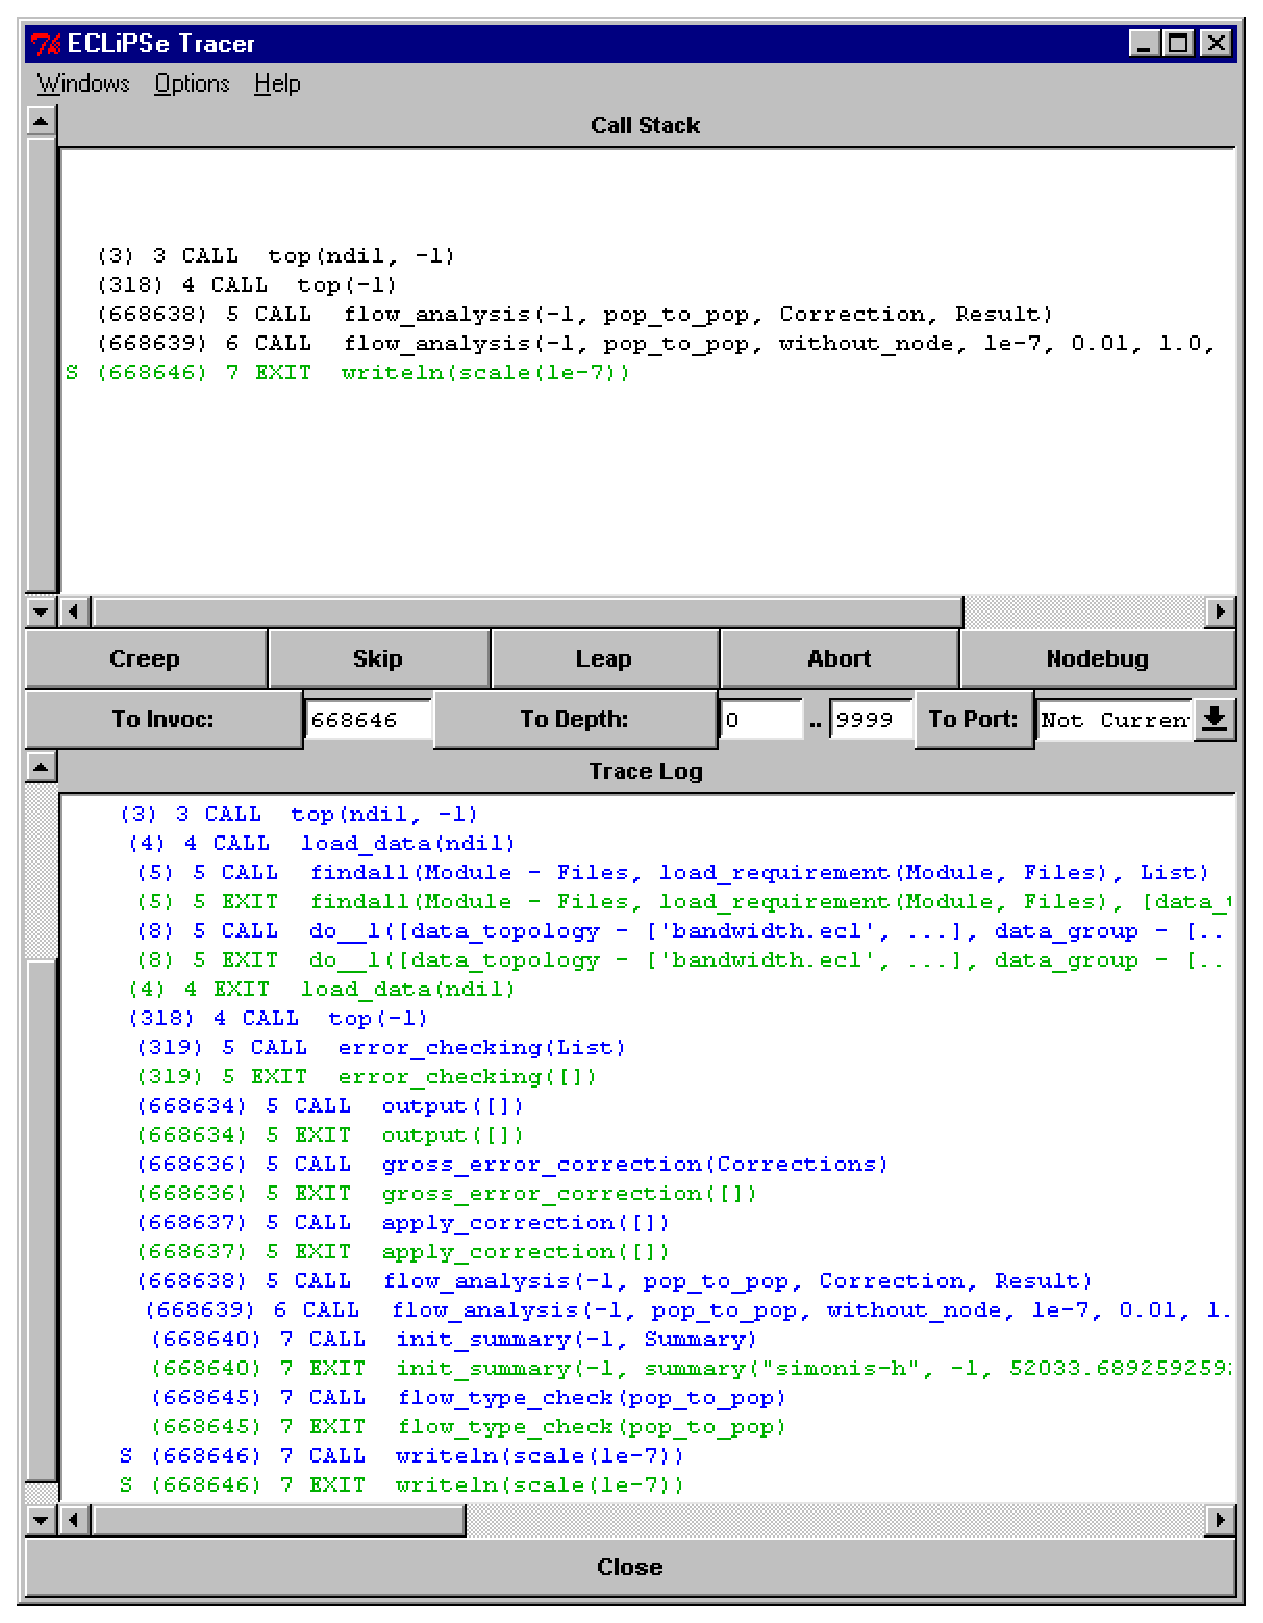
\includegraphics{tracer}}
\end{center}
\caption{\label{Tracer}ECLiPSe Tracer}
\end{figure}

\subsection{Tracing}
The three buttons {\it Creep}\index{creep}, {\it Skip}\index{skip}, {\it Leap}\index{leap} show the main commands of the tracer. The creep operation single-steps to the next statement in the program. The skip operation executes the current query and stops again when that query either succeeds or fails. The leap operation continues execution until it reaches a spy point\index{spy point}, a predicate call for which we have indicated some interest before.

A normal debugging session consists of a sequence of leap, skip and creep operations to reach an interesting part of the program and then a more detailed step-by step analysis of what is happening. It is pointless and very time consuming to single-step through a part of the program that we have already checked, but we have to be careful not to skip over the interesting part of the program.

\subsection{Jumping to a program point}
In a large program, it may be difficult to leap directly to the interesting part of the program. But we may have to repeat this operation several times, if we repeatedly leap/skip over an interesting statement. We can use the invocation number of a statement to jump\index{jump} to this exact place in the execution again. The invocation number\index{invocation number} is printed in parentheses at the beginning of each trace line. By re-starting the debugger, copying this number into the text field to the right of the button {\it To Invoc:}\index{To Invoc} and then pressing this button we can directly jump to this location.

Unfortunately, jumping to an invocation number can be quite slow in a large program. The debugger has to scan each statement to check its invocation number. It can be faster (but more tedious) to use skip and leap commands to reach a program point\footnote{Experiment! Your mileage may vary!}.

\chapter{Correctness and Performance}
\label{correctnessandperformance}

The effort in design and implementation is aimed at producing a working and maintainable program with minimal effort. But how do we check that a program is actually working?

We typically define what a correct program should do only in an informal way, stating constraints that should be satisfied, data formats that should be accepted, etc. Proving correctness\index{correctness} would require a much more formal approach, where we first agree on a specification in a formal language and then prove that the implementation satisfies that specification. But even that does not protect us from a misunderstanding in defining the spec itself, which may not reflect the wishes of the user.

Lacking this formal approach, the best hope of checking correctness of a program lies in exercising it with different types of tests.

Related to the question of correctness is the issue of performance\index{performance}. The program should not only produce correct results, but must produce them within a limited time. The correct result which is available after five years of computation is (most of the time) as useless as the wrong result obtained in five seconds.

\section{Testing}
Testing\index{testing} is often one of the activities that gets dropped when delivery time points get closer. This is a sad mistake, as any problem that is not recognized immediately will take much more effort to find and correct later on. In an ideal world, tests for each component are defined before implementation and cover each level of the design. In the real world we must find the right compromise between spending time on defining tests in the beginning and time spent on developing the application core.

A test may have different objectives:
\begin{itemize}
\item The weakest form is a test that is run to check if a program works with the test data, i.e. produces some answer without generating an error. We have suggested this form of test above to check an (incomplete) early implementation. 
\item A more complex test can be used to exercise all (or nearly all) of the program code. The test data must contain enough variation to force all alternative parts in the program. This can be achieved either by accumulating large number of tests or by designing particular tests to handle special cases.
\item Another test form is {\it regression}\index{regression testing} testing. This form of testing is used to evaluate results of a program run after each modification of the code. Results of previous runs are used to check the current results. This does not check for correctness, but rather for the same answer before and after a change.
\item {\it Correctness}\index{correctness} of a program can only be checked if we have obtained the expected results of a test in an independent way, either by hand or by a trusted program, or simply by re-using benchmark sets from a third party.
\item We may also be using some tests to do {\it performance testing}\index{performance testing}, i.e. to check that the program finds the solution within given limits on execution time and/or system resources. Clearly, this only makes sense if we also check the result for correctness. 
\end{itemize}

It is important to realize the limitations of the tests that we perform. If we have never checked that the solutions produced by a regression test are correct, then they will be most likely {\it not} correct. We only know that they are still the same solutions that the program has found before.

Unfortunately, testing of combinatorial problem\index{combinatorial problems} solvers is even more complex than testing of ``normal'' programs. Often, a given problem has more than one solution, and it is not clear in which order the answers will be produced. Providing one solution may not be enough, but there may be millions of solutions in total.

\section{Profiling}
The line profiling\footnote{The profiling facility is now available as one of the ECLiPSe libraries in the library coverage. The actual output looks slightly different.}\index{line profiling}\index{profiling} tool that we already mentioned above can be used to check the coverage\index{coverage} of the program with some query. We can easily find lines that are not executed at all, indicating the need for another test case. If we cannot construct a test which executes a program segment, then this indicates some problem.

We can use the same profile to find program parts which are executed very often and this can provide hints for optimization. Normally it is better not just to concentrate on those parts that are called very often, but on those which are calling these predicates. 

\begin{figure}[thbp]
%\psfig{figure=profile.eps,width=13.7cm}
\begin{center}
\resizebox{0.8\textwidth}{!}{\includegraphics{profile}}
\end{center}
\caption{\label{Profiling}Profiling Example}
\end{figure}

Figure \ref{Profiling} shows the output of the profiling tool. Each line is marked with the number of times it is executed (the first number in green) and the number of times we backtrack over this line (the second number in red). In this example shown there are two parts of if-then-else predicates which have not been selected by the test example.

\section{Reviewing}
A standard technique to check for consistency in the development is a reviewing\index{reviewing} process. Each module of an application goes through a review process, where persons not connected with the development check the deliverables (source code and documentation) for completeness and consistency. This review process serves multiple purposes:
\begin{itemize}
\item It forces the developer to finish a version of the program with a certain polish. 
\item It helps to find inconsistencies or missing explanations in the documentation.
\item It encourages ``best practice''\index{best practice} in the ECLiPSe application development, bringing together experts from different application teams.
\item It helps spread knowledge about applications and their sub-systems, so that re-use opportunities are recognized earlier.
\end{itemize}
On the other hand, a number of problems are normally not recognized by a review:
\begin{itemize}
\item The review checks one version of an application at a given time point. It does not guarantee that changes and modifications after the review are performed to the same standard.
\item A successful code review does not imply that the application code is correct. Reviewers might sometimes note suspect code, but a review cannot replace proper testing.
\item If nobody actually checks the code, then the whole process becomes useless overhead. This means that resources must be properly allocated to the review, it is not a task that reviewers can undertake in their spare time.
\item Comments and change requests in the review must be recorded and acted on. A formal review comment form may be used, alternatively we might work with detailed and complete minutes.
\end{itemize}

\section{Issues to check for}
\subsection{Unwanted choicepoints}
It is important to remove all unwanted choicepoints\index{choicepoint}\index{unwanted choicepoint} in an application, since they are a common source of errors. In addition, a choicepoint requires a significant amount of memory, so that leaving unwanted choicepoints is also a performance problem.

For most predicates, in particular those following one of the programming concepts in chapter \ref{programmingconcepts}, it is quite simple to avoid unwanted choicepoints. Other predicates may need more effort. We can use the ECLiPSe debugger to detect if there are any unwanted choicepoints. In the trace output for the {\it EXIT} \index{EXIT}port ECLiPSe will print a \verb+*+ if the predicate leaves a choicepoint. We can easily check a complete query by skipping over its execution and checking the exit port. If a choicepoint is indicated, we can re-run the query to locate the missed choicepoint. 

\subsection{Open streams}
A common error is to open some file without closing it before leaving. This typically happens if it is opened in one part of the program and closed in another part. Normally everything works fine, but under some exceptional circumstances the second part is not executed, leaving the file open. This can consume system resources quite quickly, leading to follow-on problems. It is a good idea to verify that every call to {\it open/3} is followed by a {\it close/1}, even if some other part of the program unexpectedly fails.

\subsection{Modified global state}
We have already stated that changing global state should be used as a last resort, not as a common practice. But if the program modifies dynamic predicates, creates global variables or uses {\it record}, then we must be very careful to restore the state properly, i.e. remove dynamic predicates after use, reset global variables etc.

\subsection{Delayed goals}
Normally, a solver should not leave delayed goals after it is finished. For some solvers, we can enforce this by instantiating all solver variables in a solution, others require more complex actions. If a query returns with delayed goals, this should be seen as an error message that needs to be investigated.
\appendix
\chapter{Style Guide}
\label{styleguide}

\section{Style rules}
\begin{enumerate}
\item   There is one directory containing all code and its documentation (using sub-directories).
\item  Filenames\index{file name} are of form [a-z][a-z\_]+ with extension .ecl .
\item  One file per module, one module per file.
\item  Each module is documented with comment directives.
\item  All required interfaces are defined in separate spec files which are included in the source with a {\it comment include} directive. This helps to separate specification and implementation code.
\item  The actual data of the problem is loaded dynamically from the Java interface; for stand-alone testing data files from the data directory are included in the correct modules.
\item  The file name is equal to the module name.
\item  Predicate names\index{predicate name} are of form [a-z][a-z\_]*[0-9]* . Underscores are used to separate words. Digits should only be used at the end of the name. Words should be English.
\item  Variable names\index{variable name} are of form [A-Z\_][a-zA-Z]*[0-9]* . Separate words star with capital letters. Words should be English. The plural should be used for lists and other collections. Digits should only be used at the end to distinguish different versions of the same conceptual thing.
\item  The code should not contain singleton variables\index{singleton}, unless their names start with \_. The final program may not generate singleton warnings.
\item  Each exported predicate is documented with a comment directive\index{comment directive}.
\item  Clauses for a predicate must be consecutive.
\item  Base clauses should be stated before recursive cases.
\item  Input arguments should be placed before output arguments.
\item  Predicates which are not exported should be documented with a single line comment. It is possible to use comment directives instead.
\item  The sequence of predicates in a file is top-down with a (possibly empty) utility section at the end.
\item  All structures are defined in one file (e.g. flow\_structures.ecl) and are documented with comment directives.
\item  Terms should not be used; instead use named structures\index{named structure}.
\item  When possible, use do loops instead of recursion.
\item  When possible, use separate predicates instead of disjunction\index{disjunction} or if-then-else.
\item  There should be no nested if-then-else\index{if then else} construct in the code.
\item  All input data should be converted into structures at the beginning of the program; there should be no direct access to the data afterwards. 
\item  All numeric constants\index{numeric constants} should be parametrized via facts. There should be no numeric values (other than 0 and 1) in rules.
\item The final code should not use failure-loops\index{failure loop}; they are acceptable for debugging or testing purposes.
\item  Cuts (!) \index{cut} should be inserted only to eliminate clearly defined choice points.
\item  The final code may not contain open choice points, except for alternative solutions that still can be explored. This is verified with the tracer tool in the debugger.
\item  Customizable data facts should always be at the end of a file; their use is deprecated.
\item  The predicate member/2\index{member/2} should only be used where backtracking is required; otherwise use memberchk/2\index{memberchk/2} to avoid hidden choice points.
\item  The final code may not contain dead code\index{dead code} except in the file/module unsupported.ecl. This file should contain all program pieces which are kept for information/debugging, but which are not part of the deliverable.
\item  The test set(s) should exercise 100 percent of the final code. Conformity is checked with the line coverage profiler.
\item  Explicit unification (=/2) should be replaced with unification inside terms where possible.
\item  There is a top-level file (document.ecl) which can be used to generated all on-line documentation automatically.
\item  Don't use ','/2 to make tuples.
\item  Don't use lists to make tuples.
\item  Avoid append/3 where possible, use accumulators instead.
\end{enumerate}

\section{Module structure}
The general form of a module is:

\begin{enumerate}
\item  module definition
\item  module comment or inclusion of a spec file
\item  exported/reexported predicates
\item  used modules
\item  used libraries
\item  local variable definitions 
\item  other global operations and settings
\item  predicate definitions
\end{enumerate}

\section{Predicate definition}
The general form of a predicate definition is:

\begin{enumerate}
\item  predicate comment directive
\item  mode declaration
\item  predicate body
\end{enumerate}

\chapter{Layout Rules}
\label{layoutrules}
In formulating these layout rules, we have taken certain arbitrary choices between different sensible formatting variants. While these choices work well for us, you may want to adapt a slightly different style. As long as it is done consistently (and agreed within a team), you should follow your own preferences.
\section{General guidelines}
Code should be indented consistently.  Tabs should be every 8 spaces.
Indentation should be one tab per level of indentation\index{indentation}, except for
highly indented code which may be indented at 4 spaces per level of
indentation after the first.

Each line should not extend beyond 79 characters, unless this is necessary
due to the use of long string literals.  If a statement or predicate call
is too long, continue it on the next line indented two levels deeper.
If the statement or call extends over more than two lines, then make sure
the subsequent lines are indented to the same depth as the second line.
For example:

\begin{verbatim}
Here is A_really_long_statement_that_does_not_fit +
           On_one_line + In_fact_it_doesnt_even_fit +
           On_two_lines.
\end{verbatim}
Don't put more than one statement or call on a line.

Put spaces after commas in comma-separated lists.  Put spaces either
side of infix operators.  In both cases, this makes them easier to read,
particularly in expressions containing long names or names with underscores.
(There are some exceptions, such as module qualification\index{module qualification} \verb^foo:bar^ and
functor/arity pairings \verb^foo/3^.  But not unification \verb^X = Y^ or list consing
\verb^[Head | Tail]^.)

Make judicious use of single blank lines in clause bodies to separate logical
components.


\section{Predicates and clauses}

Keep all clauses of a predicate\index{predicate}\index{clause} in the one place.  Leave at least one
blank line between the clauses of one predicate and the next (particularly
if they have similar names), since otherwise they may at first glance
appear to be all from the same predicate (of course, this never happens
because there's a comment before every predicate, right?).  Similarly,
it is best not to leave blank lines between the clauses of a predicate
(particularly if done inconsistently), since otherwise at first glance
they may appear to be from different predicates.

Clause heads should be flush against the left margin.  As well as making
them easier to pick out visually, this makes it easier to grep for the
definitions of predicates (as opposed to their invocations).  The head/body
separator `:-' should follow the head on the same line.  The body of the
clause should then commence on the next line, indented one tab stop.

\begin{verbatim}
non_overlap(Start1, Dur1, Start2, _Dur2):-
        Start1 + Dur1 #=< Start2.
non_overlap(Start1, _Dur1, Start2, Dur2):-
        Start1 #>= Start2 + Dur2.
\end{verbatim}

\section{If-then-elses}

If-then-elses\index{if then else, formatting} should always be parenthesised. Always include the else part, even if you don't think
it's required. Always put semicolons at the start of a new line, aligned
with the opening and closing parentheses.  Example:

\begin{verbatim}
( test1 ->
       goal1
;
       goal2
),
\end{verbatim}
\section{Disjunctions}

Disjunctions\index{disjunction, formatting} should be formatted in a similar way.  Example:

\begin{verbatim}
(
        goal1
;
        goal2
).
\end{verbatim}

\section{Do loops}

Do loops\index{do loop, formatting} should also always be parenthesised.  Loop conditions should be
listed one per line, starting after the opening parenthesis
and indented one character.  The `do' keyword should be at the end of the last condition.  The body of the
loop should then follow on the next line, again indented.  Example:

\begin{verbatim}
(for(J, I + 1, N),
 param(A, I) do
        Diff is J - I,
        A[I] #\= A[J],
        A[I] #\= A[J] + Diff,
        A[I] #\= A[J] - Diff
).
\end{verbatim}

\section{Comments}

Every predicate should have a one line comment\index{comment} documenting what it does, 
all module interfaces should be properly documented with a comment directive\index{comment directive}.

If an individual clause is long, it should be broken into sections, and
each section should have a {\it block comment}\index{block comment} describing what it does; blank
lines should be used to show the separation into sections.  Comments should
precede the code to which they apply, rather than following it.

\begin{alltt}
%
% This is a block comment; it applies to the code in the next
% section (up to the next blank line).
%
        blah,
        blah,
        blahblah,
        blah,
\end{alltt}

If a particular line or two needs explanation, a {\it line} comment\index{line comment} 

\begin{alltt}
        % This is a "line" comment; 
        % it applies to the next line or two
        % of code
        blahblah
\end{alltt}

or an {\it inline} comment\index{inline comment} 

\begin{alltt}
        blahblah        % This is an "inline" comment
\end{alltt}

should be used.

\chapter{Core Predicates}
\label{corepredicates}

This section lists essential ECLiPSe built-in and library predicates. These predicates are used in most applications, and should be well understood. There are more than 1000 other built-in and library predicates which are required for specific tasks only. 
\section{Modules}
\begin{description}
\item[module directive]\index{module directive} define a module
\item[export directive]\index{export directive} make predicates available outside a module
\item[use\_module directive]\index{use\_module directive} make predicates from other module available
\item[lib directive]\index{lib directive} make predicates from library available
\item[:] call a predicate from a particular module
\end{description}

\section{Predicate definition}
\begin{description}
\item[mode directive]\index{mode directive} define input/output modes for a predicate
\item[comment directive]\index{comment directive} define comments about a module or a predicate
\end{description}

\section{Control}
\begin{description}
\item[,] conjunction\index{conjunction}, and
\item[;] disjunction\index{disjunction}, or
\item[-\gt] implication\index{implication}, if-then-else\index{if then else} together with disjunction
\item[!] cut\index{cut}, remove choices
\item[call/1] \index{call/1}call argument as a predicate call
\item[once/1] \index{once/1}call argument as a predicate call, find one solution only
\item[not/1] \index{not/1}negation\index{negation}, fail if call to argument succeeds
\item[true/0] \index{true/0}always succeed, empty predicate definition
\item[block/3] \index{block/3}define a block in order to catch exceptions
\item[exit\_block/1] \index{exit\_block/1}jump out of a block
\end{description}

\subsection{Do Loops}
\begin{description}
\item[do] \index{do loop}general iteration operator
\item[foreach] \index{foreach}iterate over each element in a list
\item[foreacharg] \index{foreacharg}iterate over each argument of a term
\item[fromto] \index{fromto}accumulator \index{accumulator}argument
\item[for] \index{for}iterate over all integers between two bounds
\item[param] \index{param}declare parameter variables which are passed into the do-loop
\end{description}

\section{I/O}
\begin{description}
\item[exists/1] \index{exists/1}succeeds if a file exists
\item[open/3] \index{open/3}open a file or a string as a stream
\item[close/1] \index{close/1}close a stream
\item[write/2] \index{write/2}write some term to a stream
\item[nl/1] \index{nl/1}write a new-line to a stream
\item[writeln/2] \index{writeln/2}write a term to a stream, followed by a new-line
\item[writeq/2] \index{writeq/2}write a term in canoncial form, so that if can be read back
\item[read/2] \index{read/2}read a term from a stream
\item[read\_string/4] \index{read\_string/4}read a string from a stream
\item[concat\_string/2] \index{concat\_string/2}build a string from a list of components
\item[phrase/3] \index{phrase/3}call DCG \index{DCG}analyzer
\item[read\_exdr/2] \index{read\_exdr/2} read a term from a file in EXDR\index{EXDR} format
\item[write\_exdr/2] \index{write\_exdr/2} write a term to a file in EXDR\index{EXDR} format
\item[flush/1] \index{flush/1} flush an output stream
\end{description}

\section{Arrays}
\begin{description}
\item[dim/2] \index{dim/2}define an array\index{array}; can also be used to find size of an array
\item[subscript/3] \index{subscript/3}get an element of an array
\end{description}

\section{Hash Tables}
\begin{description}
\item[hash\_create/1] \index{hash\_create/1}create a hash table
\item[hash\_add/3] \index{hash\_add/3}add an item to a hash table
\item[hash\_find/3] \index{hash\_find/3}find if an item is in a hash table
\end{description}

\section{Arithmetic}
\begin{description}
\item[is/2] \index{is/2}evaluate term
\item[=:= /2] evaluate two terms and compare for equality
\item[=\bsl= /2] evaluate two terms and compare for disequality
\item[\gt /2] evaluate two terms and compare for inequality
\item[\gt= /2] evaluate two terms and compare for inequality
\item[\lt /2] evaluate two terms and compare for inequality
\item[=\lt /2] evaluate two terms and compare for inequality
\end{description}

\section{Terms and structures}
\begin{description}
\item[struct/1] \index{struct/1}define named structure
\item[with] \index{with}access element(s) in named structure
\item[of] \index{of}find argument position in named structure
\item[functor/3] \index{functor/3}define/analyze term for functor and arity
\item[arg/3] \index{arg/3}access argument of term
\item[compare/3]  \index{compare/3}compare two terms for lexicographical order
\item[= /2] two terms can be unified
\item[== /2] two terms are identical
\item[\bsl= /2] two terms cannot be unified
\item[number/1] \index{number/1}argument is a number
\item[integer/1] \index{integer/1}argument is an integer
\item[atom/1] \index{atom/1}argument is an atom
\item[var/1] \index{var/1}argument is a variable
\item[string/1] \index{string/1}argument is a string
\item[real/1] \index{real/1}argument is a float
\item[compound/1] \index{compound/1}argument is a term
\end{description}

\section{List Handling}
\begin{description}
\item[sort/2/4] \index{sort/2/4}sort a list
\item[memberchk/2] \index{memberchk/2}check if an item occurs in a list
\item[length/2] \index{length/2}find the length of a list or create a list with given length
\item[findall/3] \index{findall/3}find all solutions to a query and return a list of all answers
\end{description}
\printindex
\end{document}


% to add a floating figure
\begin{figure}[htbp]
\begin{verbatim}
\end{verbatim}
\caption{\label{}}
\end{figure}

% to add a programming concept section
\section{}
\paragraph{Description}
\paragraph{Parameters}
\begin{description}
\item[]
\end{description}
\begin{figure}[htbp]
\begin{verbatim}
\end{verbatim}
\caption{\label{}}
\end{figure}
\paragraph{Comments}
\paragraph{Example}


